\documentclass[11pt]{article}
\makeatletter\def\input@path{{../}}\makeatother
\usepackage{preamble}
\renewcommand{\chaptername}{Chapter 3: Computational approaches}
\graphicspath{{figures/}}

% ---- JAGS results (3 chains, 5,000 burn-in + 20,000 draws each), produced by
%      ch03/code/ch03_jags.R on GitHub Actions.
\newenvironment{jagsbox}{\begin{sanity}\small\textbf{JAGS output} (run on GitHub Actions; 3 chains).\par\smallskip\centering}{\end{sanity}}

\newcommand{\JAGSexfour}{\begin{jagsbox}
\begin{tabular}{l|ccc|ccc}\toprule
 & \multicolumn{3}{c|}{$a=10$} & \multicolumn{3}{c}{$a=1$}\\
 & JAGS mean & own Gibbs & $\hat R$ & JAGS mean & own Gibbs & $\hat R$\\\midrule
$b$ & 30.26 & 30.35 & 1.00 & 5.55 & 5.56 & 1.00\\
$\sigma_1^2$ & 3.24 & 3.25 & 1.00 & 12.1 & 11.6 & 1.07\\
$\sigma_{10}^2$ & 8.46 & 8.50 & 1.00 & 107 & 112 & 1.02\\\bottomrule
\end{tabular}\par\smallskip
The results agree. For $a=1$ even JAGS shows $\hat R$ slightly above 1 and posterior SDs of 82 and 563 for $\sigma_1^2,\sigma_{10}^2$: the heavy tails make means of $\sigma_i^2$ hard to estimate, exactly as discussed in (d).
\end{jagsbox}}

\newcommand{\JAGSexfive}{\begin{jagsbox}
\begin{tabular}{lccc|c}\toprule
 & JAGS mean & JAGS 95\% interval & $\hat R$ & own Gibbs mean\\\midrule
$\mu$ & 10.010 & (9.40, 10.62) & 1.00 & 10.005\\
$\delta$ & 1.191 & (0.34, 2.04) & 1.00 & 1.199\\
$\sigma$ & 2.158 & (1.88, 2.49) & 1.00 & 2.157\\\bottomrule
\end{tabular}\par\smallskip
Identical up to Monte Carlo error.
\end{jagsbox}}

\newcommand{\JAGSexseven}{\begin{jagsbox}
\begin{tabular}{lcc|lcc}\toprule
 & JAGS & own & & JAGS & own\\\midrule
Westbrook & 0.847 & 0.847 & Curry & 0.902 & 0.902\\
Harden & 0.818 & 0.819 & Antetokounmpo & 0.753 & 0.753\\
Leonard & 0.878 & 0.878 & Wall & 0.802 & 0.802\\
James & 0.677 & 0.678 & Davis & 0.788 & 0.788\\
Thomas & 0.907 & 0.908 & Durant & 0.869 & 0.869\\
\multicolumn{6}{c}{$m$: JAGS 5.60 (3.39, 9.02), own 5.66 (3.35, 9.28); all $\hat R\le1.002$}\\\bottomrule
\end{tabular}\par\smallskip
The two algorithms return the same posterior means to three decimals.
\end{jagsbox}}

\newcommand{\JAGSexnine}{\begin{jagsbox}
\begin{tabular}{lccc}\toprule
 & Mean & 95\% interval & $\hat R$\\\midrule
$\mu$ & 21{,}120 & (20{,}490, 21{,}760) & 1.000\\
$\sigma$ & 2{,}268 & (1{,}651, 3{,}057) & 1.000\\
$k$ & 2.16 & (1.25, 3.82) & 1.004\\\bottomrule
\end{tabular}\par\smallskip
Same answer as our sampler.
\end{jagsbox}}

\newcommand{\JAGSexeleven}{\begin{jagsbox}
\begin{tabular}{lcccc}\toprule
 & Mean & 95\% interval & $\hat R$ & ESS\\\midrule
$\lambda_R$ & 0.200 & (0.184, 0.217) & 1.00 & 34{,}820\\
$\lambda_{WS}$ & 0.407 & (0.205, 0.681) & 1.00 & 29{,}250\\
ratio & 2.04 & (1.02, 3.43) & 1.00 & 29{,}530\\\bottomrule
\end{tabular}
\end{jagsbox}}

\newcommand{\JAGSextwelve}{\begin{jagsbox}
\begin{tabular}{lcccc}\toprule
 & Mean & 95\% interval & $\hat R$ & ESS\\\midrule
$\alpha$ & 3.971 & (3.666, 4.270) & 1.001 & 5{,}071\\
$\beta$ & $-0.181$ & $(-0.271,\ -0.094)$ & 1.001 & 5{,}116\\\bottomrule
\end{tabular}\par\smallskip
$\Prob(\beta<0\mid\mathbf Y)=0.99997$.
\end{jagsbox}}

\newcommand{\JAGSexfourteen}{\begin{jagsbox}
Posterior means $p=(0.519,\ 0.598,\ 0.539)$; mean of \texttt{low\_best} $=\Prob(\text{low dose best})=0.739$; all $\hat R=1.00$.
\end{jagsbox}}

\newcommand{\JAGSexfifteen}{\begin{jagsbox}
$\theta$: mean 4.169, SD 0.336, 95\% interval (3.51, 4.82), $\hat R=1.00$ --- the same as the $k=2$ curve in (d).
\end{jagsbox}}

\newcommand{\JAGSexseventeen}{\begin{jagsbox}
\begin{tabular}{lcccc}\toprule
 & Mean & 95\% interval & $\hat R$ & ESS (of 150{,}000)\\\midrule
$\theta_1$ & $-15.7$ & $(-211,\ 179)$ & 1.000 & 88{,}330\\
$\theta_2$ & 235 & (24, 1{,}183) & \textbf{1.153} & \textbf{159}\\
$\theta_3$ & 1.10 & (0.35, 1.66) & 1.027 & 228\\
$\sigma$ & 795 & (360, 1{,}867) & 1.022 & 973\\\bottomrule
\end{tabular}\par\smallskip
JAGS has the same trouble: $\hat R=1.15$ for $\theta_2$ signals that the chains have \emph{not} converged, and the mean of $\theta_2$ (235 vs.\ our 354) is unstable because of its long right tail.
\end{jagsbox}}

\newcommand{\JAGSexeighteen}{\begin{jagsbox}
\begin{tabular}{lcc|cc}\toprule
 & \multicolumn{2}{c|}{$a=b=1$} & \multicolumn{2}{c}{$a=b=10$}\\
 & mean & ESS & mean & ESS\\\midrule
$n$ & 12.03 & 19{,}710 & 14.12 & 42{,}530\\
$p$ & 0.798 & 18{,}770 & 0.588 & 42{,}280\\
$\theta$ & 9.40 & 75{,}640 & 8.22 & 80{,}730\\\bottomrule
\end{tabular}\par\smallskip
Same pattern: the informative prior on $p$ more than doubles the ESS of $n$ and $p$.
\end{jagsbox}}

\newcommand{\JAGSexnineteen}{\begin{jagsbox}
\begin{tabular}{cc|ccc}\toprule
$n$ & $\epsilon$ & ESS $\theta_1$ & ESS $\theta_2$ & ESS $\theta_3$\\\midrule
5 & 0.1 & 983 & 144 & 338\\
5 & 10 & 8{,}777 & 6{,}355 & 13{,}260\\
25 & 0.1 & 7{,}967 & \textbf{12} & 104\\
25 & 10 & 5{,}202 & 10{,}691 & 15{,}018\\\bottomrule
\end{tabular}\par\smallskip
(One chain of 20{,}000 draws each.) JAGS shows the same pattern as our sampler.
\end{jagsbox}}

\begin{document}

\solutionstitlepage{3}{Computational approaches}{All numbers and figures are reproduced by \texttt{ch03/code/ch03.R} (hand-written samplers, base R). The JAGS versions are in \texttt{ch03/code/ch03\_jags.R}; they run automatically on GitHub.}

\tableofcontents
\clearpage

% ================================================================= primer
\section*{A five-minute primer on the tools of this chapter}
\addcontentsline{toc}{section}{Primer: the tools of this chapter}

Almost every exercise in this chapter uses one of the following ideas. Read this page once; the solutions refer back to it.

\begin{recall}
\textbf{1. The posterior up to a constant.} Bayes' rule says
$p(\theta\mid\mathbf Y)=\dfrac{f(\mathbf Y\mid\theta)\pi(\theta)}{m(\mathbf Y)}$. The denominator $m(\mathbf Y)$ does not depend on $\theta$, so we usually write
\[
p(\theta\mid\mathbf Y)\ \propto\ f(\mathbf Y\mid\theta)\,\pi(\theta)\qquad(\text{``likelihood}\times\text{prior''}).
\]
We work on the \emph{log scale}, $\log p=\log f+\log\pi+\text{const}$, because products become sums and numbers stay in a safe range.

\medskip
\textbf{2. MAP estimate.} The \emph{maximum a posteriori} estimate is the peak of the posterior: solve $\frac{\dd}{\dd\theta}\log p(\theta\mid\mathbf Y)=0$.

\medskip
\textbf{3. Bayesian CLT.} With enough data the posterior is approximately normal, centred at the MAP, with variance equal to the inverse of the curvature:
\[
\theta\mid\mathbf Y\ \approx\ \dist{Normal}\Big(\hat\theta_{MAP},\ \big[-\tfrac{\dd^2}{\dd\theta^2}\log p(\theta\mid\mathbf Y)\big|_{\hat\theta}\big]^{-1}\Big).
\]

\medskip
\textbf{4. Full conditional distribution.} For a model with several parameters, the full conditional of one parameter is its distribution \emph{given the data and all the other parameters}. Recipe: write the joint ``likelihood $\times$ prior'', keep only the factors that contain the parameter, and recognise the shape.

\medskip
\textbf{5. Gibbs sampling.} Start somewhere; then repeatedly draw each parameter from its full conditional, using the latest values of the others. After a burn-in period, the draws behave like (correlated) draws from the posterior.

\medskip
\textbf{6. Metropolis--Hastings (random walk).} When a full conditional has no standard form: propose $\theta^*=\theta+\text{noise}$, compute
\[
R=\frac{p(\theta^*\mid\mathbf Y)}{p(\theta\mid\mathbf Y)}\quad(\text{only ratios needed --- the unknown constant cancels}),
\]
accept $\theta^*$ with probability $\min(1,R)$, otherwise keep $\theta$. The noise size (step) is tuned so that roughly 30--50\% of proposals are accepted.

\medskip
\textbf{7. Convergence diagnostics.}
\emph{Trace plot}: the chain should look like a ``hairy caterpillar'' with no trend. \emph{$\hat R$ (Gelman--Rubin)}: run several chains from different starting points; $\hat R\approx1$ (below 1.01--1.1) means they agree. \emph{Effective sample size (ESS)}: the number of independent draws the correlated chain is worth; aim for at least a few hundred to a thousand.
\end{recall}

\clearpage

% ================================================================= Exercise 1
\exercise{3.1 --- Pros and cons of five computational methods}

\begin{problem}{1}
Give an advantage and a disadvantage of the following methods:
\begin{enumerate}[(a)]
\item Maximum a posteriori estimation
\item Numerical integration
\item Bayesian central limit theorem
\item Gibbs sampling
\item Metropolis--Hastings sampling
\end{enumerate}
\end{problem}

\begin{restate}
For each way of ``computing a posterior'', say one thing it does well and one thing it does badly.
\end{restate}

\begin{keyidea}
Ask two questions of every method: \emph{(i) how much of the posterior does it give me} (a single number? the whole distribution?), and \emph{(ii) how does it cope as the number of parameters grows?}
\end{keyidea}

\solution
\begin{center}
\small
\renewcommand{\arraystretch}{1.35}
\begin{tabular}{p{0.17\linewidth}p{0.37\linewidth}p{0.37\linewidth}}\toprule
Method & \textbf{Advantage} & \textbf{Disadvantage}\\\midrule
(a) MAP & Fast: only an optimisation problem (works for thousands of parameters); no integration needed. & Gives a single point, \emph{no uncertainty}; the mode can be unrepresentative of a skewed or multi-modal posterior.\\
(b) Numerical integration & Very accurate (essentially exact) posterior means, probabilities and plots for 1--2 parameters; no randomness. & Cost explodes with dimension (a grid of 100 points per parameter needs $100^p$ evaluations) --- impossible beyond 3--4 parameters.\\
(c) Bayesian CLT & Only needs the MAP and the curvature; gives an instant normal approximation with standard errors. & Only valid for large samples; wrong for skewed posteriors, small $n$, or parameters near a boundary.\\
(d) Gibbs sampling & No tuning: each step is an exact draw from a known distribution, and it scales to many parameters. & Needs every full conditional to be a recognisable distribution; mixes very slowly when parameters are strongly correlated.\\
(e) Metropolis--Hastings & Works for \emph{any} posterior we can evaluate up to a constant (no conjugacy needed). & Must be tuned (step size); poor tuning gives highly correlated draws, and it struggles in high dimensions.\\\bottomrule
\end{tabular}
\end{center}

\begin{answer}
See the table: deterministic methods (a)--(c) are fast/accurate but either lose uncertainty or do not scale; sampling methods (d)--(e) give the full posterior in high dimensions but need checking and/or tuning.
\end{answer}

\begin{takeaway}
In practice they are combined: MAP gives starting values, the CLT gives proposal step sizes, and MCMC does the final job.
\end{takeaway}

% ================================================================= Exercise 2
\exercise{3.2 --- MAP and posterior mean with known variances}

\begin{problem}{2}
Assume that $Y_i|\mu\overset{indep}{\sim}\dist{Normal}(\mu,\sigma_i^2)$ for $i\in\{1,\dots,n\}$, with $\sigma_i$ known and improper prior distribution $\pi(\mu)=1$ for all $\mu$.
\begin{enumerate}[(a)]
\item Give a formula for the MAP estimator for $\mu$.
\item We observe $n=3$, $Y_1=12$, $Y_2=10$, $Y_3=22$, $\sigma_1=\sigma_2=3$ and $\sigma_3=10$; compute the MAP estimate of $\mu$.
\item Use numerical integration to compute the posterior mean of $\mu$.
\item Plot the posterior distribution of $\mu$, and indicate the MAP and the posterior mean estimates on the plot.
\end{enumerate}
\end{problem}

\begin{restate}
Three measurements of the same quantity $\mu$ have different accuracies (the third is much noisier). Find the most likely value of $\mu$, then its posterior mean, and draw the posterior.
\end{restate}

\begin{recall}
The normal density is $\dfrac{1}{\sqrt{2\pi}\sigma}\exp\Big\{-\dfrac{(y-\mu)^2}{2\sigma^2}\Big\}$. Its log is $-\dfrac{(y-\mu)^2}{2\sigma^2}+\text{(terms without }\mu)$.
\end{recall}

\begin{keyidea}
With a flat prior, the posterior is proportional to the likelihood, so the MAP is the maximum-likelihood estimate --- a \textbf{precision-weighted average} in which accurate measurements count more.
\end{keyidea}

\solution
\step{(a) Step 1 --- write the log posterior.}
With $\pi(\mu)=1$, $\log\pi=0$, so
\[
\log p(\mu\mid\mathbf Y)=\sum_{i=1}^n\log f(Y_i\mid\mu)+\text{const}=-\sum_{i=1}^n\frac{(Y_i-\mu)^2}{2\sigma_i^2}+\text{const}.
\]

\step{(a) Step 2 --- differentiate and set to zero.}
\[
\frac{\dd}{\dd\mu}\log p=\sum_{i=1}^n\frac{2(Y_i-\mu)}{2\sigma_i^2}=\sum_{i=1}^n\frac{Y_i-\mu}{\sigma_i^2}=0.
\]
\why{The derivative of $-(Y_i-\mu)^2$ with respect to $\mu$ is $+2(Y_i-\mu)$ (chain rule: the inner derivative of $Y_i-\mu$ is $-1$).}

\step{(a) Step 3 --- solve for $\mu$.}
Write $w_i=1/\sigma_i^2$ (the \emph{precision} of measurement $i$). Then $\sum_iw_iY_i-\mu\sum_iw_i=0$, so
\[
\hat\mu_{MAP}=\frac{\sum_{i=1}^nw_iY_i}{\sum_{i=1}^nw_i},\qquad w_i=\frac1{\sigma_i^2}.
\]

\step{(a) Step 4 --- check it is a maximum.}
$\frac{\dd^2}{\dd\mu^2}\log p=-\sum_iw_i<0$, so the curve bends down: a maximum.

\step{(b) Plug in the numbers.}
\[
w_1=w_2=\tfrac19=0.1111,\qquad w_3=\tfrac1{100}=0.01,\qquad\sum w_i=0.2322,
\]
\[
\sum w_iY_i=\tfrac{12}{9}+\tfrac{10}{9}+\tfrac{22}{100}=1.3333+1.1111+0.2200=2.6644,
\qquad
\hat\mu_{MAP}=\frac{2.6644}{0.2322}=\mathbf{11.474}.
\]
\why{The noisy third value (22) gets less than 5\% of the total weight, so the estimate sits close to the average of 12 and 10.}

\step{(c) Numerical integration.}
Evaluate the unnormalised posterior $g(\mu)=\exp\{\log p(\mu\mid\mathbf Y)\}$ on a fine grid $\mu_1<\dots<\mu_G$ (5{,}001 points from 0 to 25, spacing $\Delta$). Then
\[
p(\mu_j\mid\mathbf Y)\approx\frac{g(\mu_j)}{\sum_kg(\mu_k)\Delta},\qquad
\E(\mu\mid\mathbf Y)\approx\sum_j\mu_j\,p(\mu_j\mid\mathbf Y)\,\Delta=\mathbf{11.474}.
\]

\step{(d) Plot.}
\begin{center}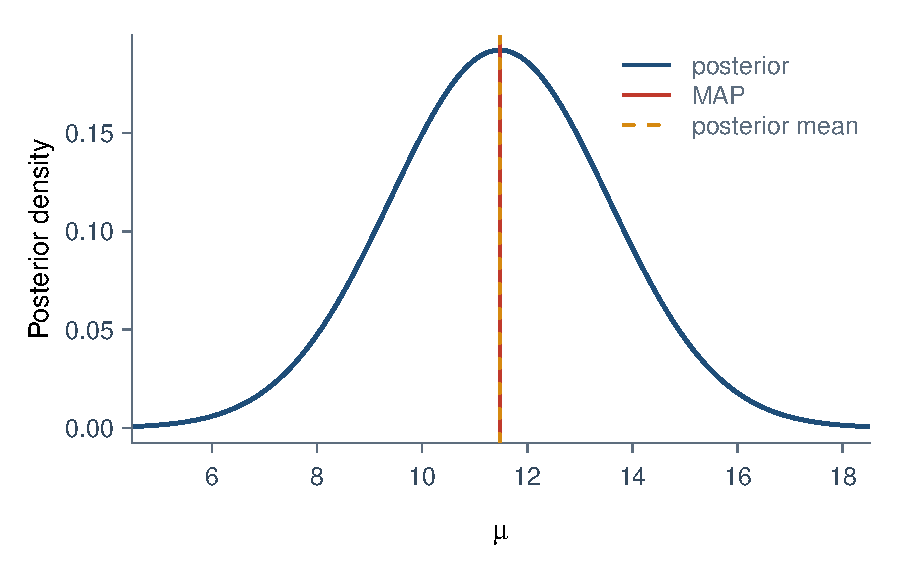
\includegraphics[width=0.66\linewidth]{ex02_map.pdf}\end{center}
The two vertical lines lie exactly on top of each other.

\begin{sanity}
The log posterior in Step 1 is a \emph{quadratic} in $\mu$, so the posterior is exactly normal:
$\mu\mid\mathbf Y\sim\dist{Normal}\big(\hat\mu_{MAP},\ 1/\sum w_i\big)=\dist{Normal}(11.474,\ 2.075^2)$. For a symmetric distribution the mode (MAP) equals the mean, which is why (b) and (c) agree.
\end{sanity}

\begin{answer}
(a) $\hat\mu_{MAP}=\sum_iY_i\sigma_i^{-2}\big/\sum_i\sigma_i^{-2}$ (precision-weighted mean). \quad (b) $11.474$. \quad (c) $11.474$. \quad (d) See the figure: the posterior is $\dist{Normal}(11.47,\,2.08^2)$.
\end{answer}

\begin{takeaway}
Never average measurements of different quality with equal weights: the simple mean $(12+10+22)/3=14.7$ is pulled far off by the least reliable value.
\end{takeaway}

% ================================================================= Exercise 3
\exercise{3.3 --- Poisson counts with exposures: MAP and the Bayesian CLT}

\begin{problem}{3}
Assume $Y_i|\lambda\overset{indep}{\sim}\dist{Poisson}(N_i\lambda)$ for $i=1,\dots,n$.
\begin{enumerate}[(a)]
\item Identify a conjugate prior for $\lambda$, and derive the posterior that follows from this prior.
\item Using the prior $\lambda\sim\dist{Uniform}(0,20)$, derive the MAP estimator of $\lambda$.
\item Using the prior $\lambda\sim\dist{Uniform}(0,20)$, plot the posterior on a grid of $\lambda$ assuming $n=2$, $N_1=50$, $N_2=100$, $Y_1=12$, and $Y_2=25$, and show that the MAP estimate is indeed the maximizer.
\item Use the Bayesian CLT to approximate the posterior of $\lambda$ under the setting of (c), plot the approximate posterior, and compare the plot with the plot from (c).
\end{enumerate}
\end{problem}

\begin{restate}
Unit $i$ has size $N_i$ (e.g.\ population or time) and produces $Y_i$ events at rate $\lambda$ per unit. Find a conjugate prior, the MAP under a uniform prior, and compare the exact posterior with its normal approximation.
\end{restate}

\begin{recall}
Poisson PMF: $\Prob(Y=y)=\dfrac{e^{-m}m^y}{y!}$ with mean $m$. Gamma density: $\pi(\lambda)\propto\lambda^{a-1}e^{-b\lambda}$, mean $a/b$, variance $a/b^2$.
\end{recall}

\begin{keyidea}
As a function of $\lambda$, the likelihood is $\lambda^{\sum Y_i}e^{-\lambda\sum N_i}$ --- a Gamma kernel. Only two numbers matter: total events $\sum Y_i$ and total exposure $\sum N_i$.
\end{keyidea}

\solution
\step{(a) Step 1 --- the likelihood as a function of $\lambda$.}
\[
f(\mathbf Y\mid\lambda)=\prod_{i=1}^n\frac{e^{-N_i\lambda}(N_i\lambda)^{Y_i}}{Y_i!}
=\underbrace{\prod_i\frac{N_i^{Y_i}}{Y_i!}}_{\text{no }\lambda}\ \lambda^{\sum Y_i}\,e^{-\lambda\sum N_i}
\ \propto\ \lambda^{\sum Y_i}e^{-\lambda\sum N_i}.
\]
\step{(a) Step 2 --- multiply by a Gamma prior.}
\[
p(\lambda\mid\mathbf Y)\propto\lambda^{\sum Y_i}e^{-\lambda\sum N_i}\cdot\lambda^{a-1}e^{-b\lambda}
=\lambda^{(a+\sum Y_i)-1}e^{-(b+\sum N_i)\lambda}.
\]
This is again a Gamma kernel, so the \textbf{Gamma prior is conjugate}:
$\lambda\mid\mathbf Y\sim\dist{Gamma}\big(a+\sum Y_i,\ b+\sum N_i\big)$.

\step{(b) MAP under $\dist{Uniform}(0,20)$.}
The prior is constant on $(0,20)$, so on that interval $\log p=S_Y\log\lambda-S_N\lambda+\text{const}$ with $S_Y=\sum Y_i$, $S_N=\sum N_i$.
\[
\frac{\dd}{\dd\lambda}\log p=\frac{S_Y}{\lambda}-S_N=0\ \Rightarrow\ \lambda=\frac{S_Y}{S_N}.
\]
Second derivative $-S_Y/\lambda^2<0$: a maximum. Because the prior cuts off at 20,
\[
\hat\lambda_{MAP}=\min\Big(\frac{\sum Y_i}{\sum N_i},\ 20\Big).
\]
\why{If the unconstrained peak were above 20, the posterior would be increasing all the way up to the boundary, so its highest point would be at 20.}

\step{(c) Numbers and grid plot.}
$S_Y=12+25=37$, $S_N=50+100=150$, so $\hat\lambda_{MAP}=37/150=\mathbf{0.2467}$. On a grid of 2{,}001 values the largest posterior value occurs at $\lambda=0.2467$ --- the same number (dotted line below).

\step{(d) Bayesian CLT.}
Curvature at the MAP: $-\frac{\dd^2}{\dd\lambda^2}\log p=\frac{S_Y}{\lambda^2}$, evaluated at $\hat\lambda$:
\[
\frac{S_Y}{\hat\lambda^2}=\frac{S_Y}{(S_Y/S_N)^2}=\frac{S_N^2}{S_Y}
\quad\Rightarrow\quad
\V\approx\frac{S_Y}{S_N^2}=\frac{37}{150^2}=0.001644,\quad\text{SD}=0.0406.
\]
So $\lambda\mid\mathbf Y\approx\dist{Normal}(0.2467,\ 0.0406^2)$.
\begin{center}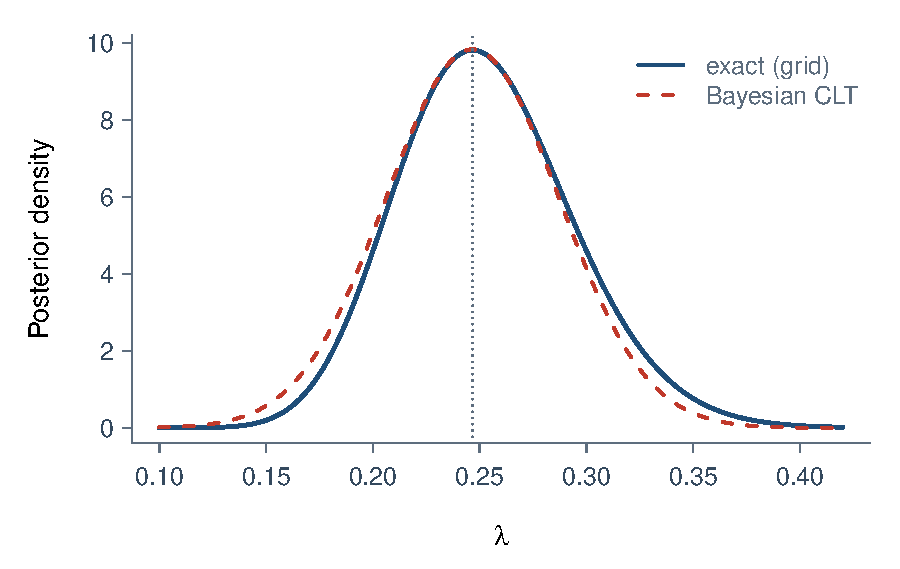
\includegraphics[width=0.68\linewidth]{ex03_clt.pdf}\end{center}
The exact posterior (a $\dist{Gamma}(38,150)$ truncated at 20) is very slightly right-skewed; the normal approximation is symmetric but otherwise almost identical.

\begin{sanity}
The exact posterior SD is $\sqrt{38}/150=0.0411$, very close to the CLT's 0.0406. With 37 events, the CLT is already accurate.
\end{sanity}

\begin{answer}
(a) $\lambda\sim\dist{Gamma}(a,b)\Rightarrow\lambda\mid\mathbf Y\sim\dist{Gamma}(a+\sum Y_i,\ b+\sum N_i)$.
(b) $\hat\lambda_{MAP}=\min(\sum Y_i/\sum N_i,\ 20)$.
(c) $\hat\lambda_{MAP}=37/150=0.2467$, confirmed as the grid maximiser.
(d) $\dist{Normal}(0.2467,\ 0.0406^2)$, nearly identical to the exact posterior.
\end{answer}

\begin{takeaway}
The CLT works well here because there are many events (37). With, say, 2 events the Gamma posterior would be clearly skewed and the normal approximation could even put mass below zero.
\end{takeaway}

% ================================================================= Exercise 4
\exercise{3.4 --- A Gibbs sampler for a hierarchical variance model}

\begin{problem}{4}
Consider the model $Y_i|\sigma_i^2\overset{indep}{\sim}\dist{Normal}(0,\sigma_i^2)$ for $i=1,\dots,n$ where $\sigma_i^2|b\sim\dist{InvGamma}(a,b)$ and $b\sim\dist{Gamma}(1,1)$.
\begin{enumerate}[(a)]
\item Derive the full conditional posterior distributions for $\sigma_1^2$ and $b$.
\item Write pseudocode for Gibbs sampling; i.e., describe in detail each step of the Gibbs sampling algorithm.
\item Write your own Gibbs sampling code (not in JAGS), and plot the marginal posterior density for each parameter. Assume $n=10$, $a=10$ and $Y_i=i$ for $i=1,\dots,10$.
\item Repeat the analysis with $a=1$, and comment on the convergence of the MCMC chain.
\item Implement this model in (c) using JAGS, and compare the results with the results in (c).
\end{enumerate}
\end{problem}

\begin{restate}
Each observation has its own variance $\sigma_i^2$; the variances share a common scale $b$. Derive the Gibbs updates, code them, and compare two values of the prior shape $a$.
\end{restate}

\begin{recall}
$X\sim\dist{InvGamma}(a,b)$ means $1/X\sim\dist{Gamma}(a,b)$, with density $\pi(x)=\frac{b^a}{\Gamma(a)}x^{-a-1}e^{-b/x}$ and mean $b/(a-1)$ for $a>1$. Its kernel in $x$ is $x^{-a-1}e^{-b/x}$; its kernel in $b$ is $b^ae^{-b/x}$.
\end{recall}

\begin{keyidea}
To find a full conditional, write the joint density and keep only the factors containing the parameter of interest. Here both full conditionals turn out to be standard distributions, so plain Gibbs works.
\end{keyidea}

\solution
\step{(a) The joint posterior.}
\[
p(\sigma_1^2,\dots,\sigma_n^2,b\mid\mathbf Y)\ \propto\ \prod_{i=1}^n\Big[\underbrace{(\sigma_i^2)^{-1/2}e^{-Y_i^2/(2\sigma_i^2)}}_{\text{likelihood}}\ \underbrace{\tfrac{b^a}{\Gamma(a)}(\sigma_i^2)^{-a-1}e^{-b/\sigma_i^2}}_{\text{prior of }\sigma_i^2}\Big]\ \underbrace{e^{-b}}_{\text{prior of }b}.
\]

\step{(a) Full conditional of $\sigma_1^2$.}
Keep only factors with $\sigma_1^2$ (the $i=1$ term):
\[
p(\sigma_1^2\mid\cdot)\propto(\sigma_1^2)^{-1/2}e^{-Y_1^2/(2\sigma_1^2)}(\sigma_1^2)^{-a-1}e^{-b/\sigma_1^2}
=(\sigma_1^2)^{-(a+\frac12)-1}\exp\Big\{-\frac{b+Y_1^2/2}{\sigma_1^2}\Big\}.
\]
\why{Add the exponents of $\sigma_1^2$: $-\frac12-a-1=-(a+\frac12)-1$; add the numerators in the exponential: $\frac{Y_1^2}{2}+b$.}
This is the inverse-gamma kernel, so
\[
\sigma_1^2\mid\cdot\ \sim\ \dist{InvGamma}\big(a+\tfrac12,\ b+\tfrac{Y_1^2}2\big)\qquad(\text{and the same for every }i).
\]

\step{(a) Full conditional of $b$.}
Keep factors with $b$: one $b^a e^{-b/\sigma_i^2}$ per observation, plus the prior $e^{-b}$:
\[
p(b\mid\cdot)\propto\prod_{i=1}^nb^ae^{-b/\sigma_i^2}\cdot e^{-b}=b^{na}\exp\Big\{-b\Big(1+\sum_i\frac1{\sigma_i^2}\Big)\Big\}
\ \Rightarrow\ b\mid\cdot\sim\dist{Gamma}\Big(na+1,\ 1+\sum_{i=1}^n\frac1{\sigma_i^2}\Big).
\]

\step{(b) Pseudocode.}
\begin{enumerate}[1.]
\item \textbf{Initialise}: $\sigma_i^{2(0)}=Y_i^2+1$ for all $i$, $b^{(0)}=1$.
\item \textbf{For} $s=1,\dots,S$:
\begin{enumerate}[(i)]
\item for $i=1,\dots,n$: draw $\sigma_i^{2(s)}\sim\dist{InvGamma}\big(a+\frac12,\ b^{(s-1)}+Y_i^2/2\big)$\\
(in R: \texttt{1/rgamma(n, a + 0.5, b + Y\^{}2/2)});
\item draw $b^{(s)}\sim\dist{Gamma}\big(na+1,\ 1+\sum_i1/\sigma_i^{2(s)}\big)$;
\item store $(\sigma_1^{2(s)},\dots,\sigma_n^{2(s)},b^{(s)})$.
\end{enumerate}
\item \textbf{Discard} the first $B$ draws (burn-in) and use the rest as posterior samples. Check trace plots and the effective sample size.
\end{enumerate}

\step{(c) Results for $a=10$} (20{,}000 iterations, first 2{,}000 discarded):
\begin{center}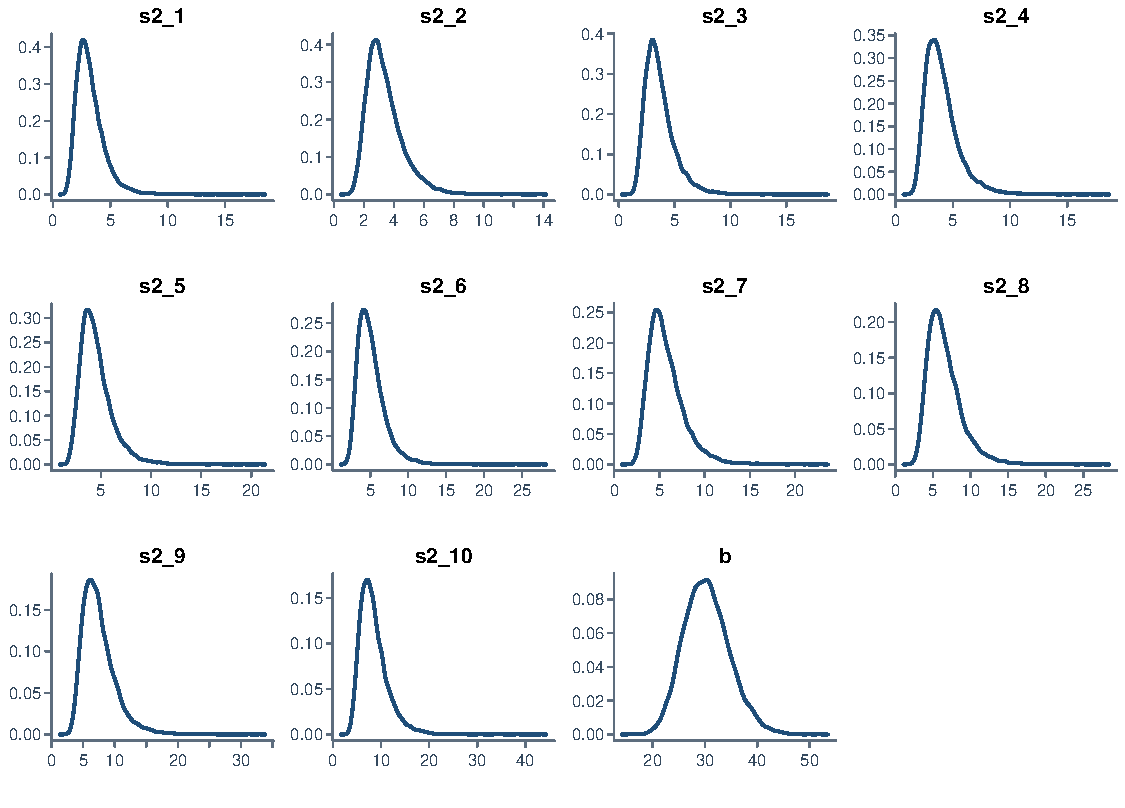
\includegraphics[width=0.98\linewidth]{ex04_marginals.pdf}\end{center}
Posterior means: $b\approx30.4$, $\sigma_1^2\approx3.25$, $\sigma_{10}^2\approx8.50$. With $a=10$ the prior is fairly tight around $b/a\approx3$, so even $Y_{10}=10$ (which on its own suggests $\sigma_{10}^2\approx100$) is pulled down to about 8.5.

\step{(d) $a=1$ and convergence.}
Posterior means: $b\approx5.6$, $\sigma_1^2\approx11.6$, $\sigma_{10}^2\approx112$. The chain itself mixes well (ESS for $b$: 10{,}451 out of 18{,}000), but the trace plot of $\sigma_{10}^2$ shows occasional huge spikes (note the very different vertical scales):
\begin{center}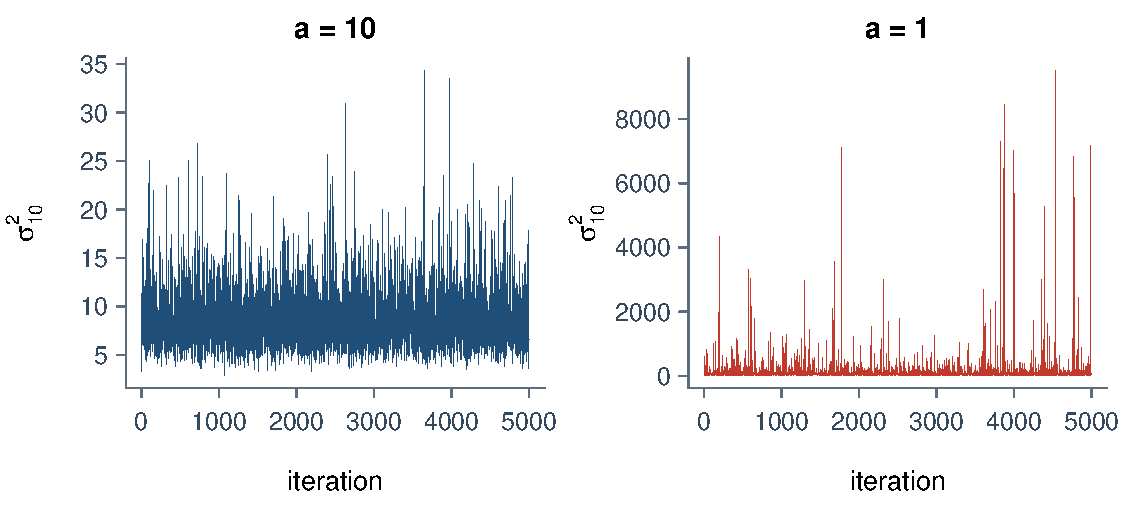
\includegraphics[width=0.9\linewidth]{ex04_traces.pdf}\end{center}
\why{With $a=1$ the full conditional of $\sigma_i^2$ is $\dist{InvGamma}(1.5,\cdot)$, which has a finite mean but an \emph{infinite variance}. Rare enormous draws are a genuine feature of the posterior, not a convergence failure --- but they make Monte Carlo averages of $\sigma_i^2$ unstable, so we need many more draws (or should report medians).}

\step{(e) JAGS.} The same model in JAGS (prior on the precision $1/\sigma_i^2\sim\dist{Gamma}(a,b)$, which is equivalent):
\begin{lstlisting}
model{
  for(i in 1:n){
    Y[i] ~ dnorm(0, prec[i])     # JAGS uses precision = 1/variance
    prec[i] ~ dgamma(a, b)       # => sigma2[i] ~ InvGamma(a, b)
    sigma2[i] <- 1 / prec[i]
  }
  b ~ dgamma(1, 1)
}
\end{lstlisting}
\JAGSexfour

\begin{answer}
(a) $\sigma_i^2\mid\cdot\sim\dist{InvGamma}(a+\frac12,\ b+\frac{Y_i^2}2)$ and $b\mid\cdot\sim\dist{Gamma}(na+1,\ 1+\sum_i\sigma_i^{-2})$.
(b) Alternate the two draws (pseudocode above). (c) $a=10$: strong pooling, $\E(b\mid\mathbf Y)\approx30$.
(d) $a=1$: weak pooling; good mixing but heavy-tailed draws of $\sigma_i^2$. (e) JAGS agrees.
\end{answer}

\begin{takeaway}
``Good mixing'' (high ESS) and ``stable averages'' are different things: if the posterior has very heavy tails, even independent draws give noisy means.
\end{takeaway}

% ================================================================= Exercise 5
\exercise{3.5 --- Gibbs sampling for a two-group comparison}

\begin{problem}{5}
Consider the model $Y_i|\mu,\sigma^2\sim\dist{Normal}(\mu,\sigma^2)$ for $i=1,\dots,n$ and $Y_i|\mu,\delta,\sigma^2\sim\dist{Normal}(\mu+\delta,\sigma^2)$ for $i=n+1,\dots,n+m$, where $\mu,\delta\sim\dist{Normal}(0,100^2)$ and $\sigma^2\sim\dist{InvGamma}(0.01,0.01)$.
\begin{enumerate}[(a)]
\item Give an example of a real experiment for which this would be an appropriate model.
\item Derive the full conditional posterior distributions for $\mu$, $\delta$ and $\sigma^2$.
\item Simulate a dataset from this model with $n=m=50$, $\mu=10$, $\delta=1$ and $\sigma=2$. Write your own Gibbs sampling code (not in JAGS) to fit the model above to the simulated data, and plot the marginal posterior density for each parameter. Are you able to recover the true values reasonably well?
\item Implement this model using JAGS, and compare the results with the results in (c).
\end{enumerate}
\end{problem}

\begin{restate}
A control group has mean $\mu$; a treatment group has mean $\mu+\delta$; both have the same noise level $\sigma$. Derive the Gibbs updates and check them on simulated data.
\end{restate}

\begin{recall}
\textbf{Completing the square.} If a log density in $x$ has the form $-\frac{A}{2}x^2+Bx+\text{const}$, then $x\sim\dist{Normal}(B/A,\ 1/A)$. So for normal full conditionals we only need to collect the coefficient of $x^2$ (the precision $A$) and of $x$ (the term $B$).
\end{recall}

\begin{keyidea}
Write $g_i=1$ for treated units and $g_i=0$ for controls, so $Y_i\sim\dist{Normal}(\mu+\delta g_i,\sigma^2)$ for every $i$. Each full conditional is normal or inverse-gamma.
\end{keyidea}

\solution
\step{(a) Example.} A clinical trial of a blood-pressure drug: $n$ patients get a placebo (mean $\mu$), $m$ get the drug (mean $\mu+\delta$); $\delta$ is the treatment effect, and the spread $\sigma$ is assumed equal in both groups. (Also: crop yield without/with a fertiliser.)

\step{(b) Full conditional of $\mu$.}
Let $N=n+m$. The terms with $\mu$ are
\[
-\frac{1}{2\sigma^2}\sum_{i=1}^N(Y_i-\delta g_i-\mu)^2-\frac{\mu^2}{2\cdot100^2}.
\]
Coefficient of $\mu^2$: $A=\frac{N}{\sigma^2}+\frac1{100^2}$. Coefficient of $\mu$: $B=\frac{1}{\sigma^2}\sum_i(Y_i-\delta g_i)$. Hence
\[
\mu\mid\cdot\sim\dist{Normal}\Big(\frac{\sum_i(Y_i-\delta g_i)/\sigma^2}{N/\sigma^2+1/100^2},\ \frac{1}{N/\sigma^2+1/100^2}\Big).
\]
\why{Expanding $(Y_i-\delta g_i-\mu)^2=\mu^2-2\mu(Y_i-\delta g_i)+\dots$; summing over $i$ and multiplying by $-\frac1{2\sigma^2}$ gives $-\frac{N}{2\sigma^2}\mu^2+\frac{\sum(Y_i-\delta g_i)}{\sigma^2}\mu$.}

\step{(b) Full conditional of $\delta$.}
Only the treated observations contain $\delta$:
\[
\delta\mid\cdot\sim\dist{Normal}\Big(\frac{\sum_{i>n}(Y_i-\mu)/\sigma^2}{m/\sigma^2+1/100^2},\ \frac{1}{m/\sigma^2+1/100^2}\Big).
\]

\step{(b) Full conditional of $\sigma^2$.}
\[
p(\sigma^2\mid\cdot)\propto(\sigma^2)^{-N/2}\exp\Big\{-\frac{\text{SSE}}{2\sigma^2}\Big\}(\sigma^2)^{-0.01-1}e^{-0.01/\sigma^2},\qquad\text{SSE}=\sum_i(Y_i-\mu-\delta g_i)^2,
\]
so $\sigma^2\mid\cdot\sim\dist{InvGamma}\big(0.01+\frac N2,\ 0.01+\frac{\text{SSE}}2\big)$.

\step{(c) Simulation and Gibbs sampler.} We simulated 50 values from $\dist N(10,2^2)$ and 50 from $\dist N(11,2^2)$, then ran 20{,}000 Gibbs iterations (1{,}000 burn-in), cycling through the three updates above.
\begin{center}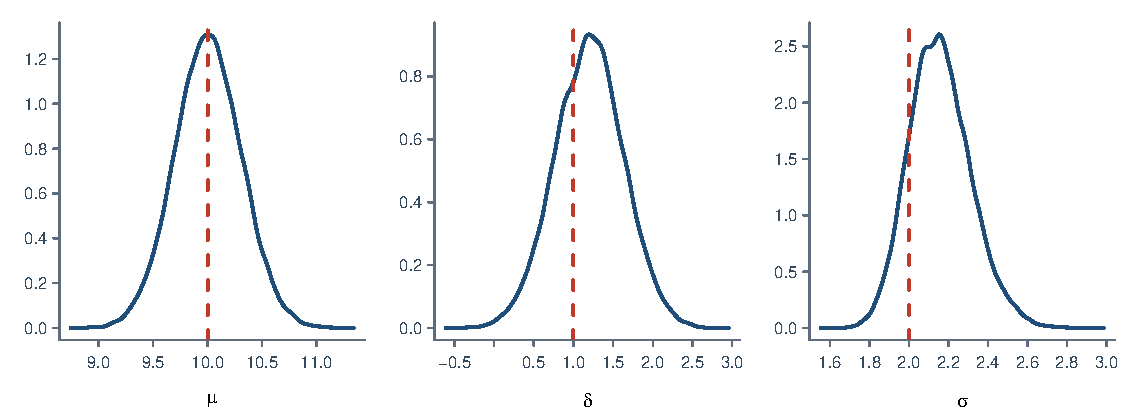
\includegraphics[width=0.98\linewidth]{ex05_marginals.pdf}\end{center}
\begin{center}
\begin{tabular}{lcccc}\toprule
Parameter & Truth & Posterior mean & SD & 95\% interval\\\midrule
$\mu$ & 10 & 10.005 & 0.305 & (9.41, 10.61)\\
$\delta$ & 1 & 1.199 & 0.431 & (0.35, 2.04)\\
$\sigma$ & 2 & 2.157 & 0.156 & (1.88, 2.49)\\\bottomrule
\end{tabular}
\end{center}
All three true values (red dashed lines) fall well inside the 95\% intervals.

\begin{sanity}
With such vague priors the posterior means should match the classical estimates: the control-group mean is 10.010, the difference in group means is 1.190 and the pooled SD is 2.141 --- essentially the same as the table.
\end{sanity}

\step{(d) JAGS.}
\begin{lstlisting}
model{
  for(i in 1:N){ Y[i] ~ dnorm(mu + delta * group[i], tau) }
  mu    ~ dnorm(0, 1 / 100^2)
  delta ~ dnorm(0, 1 / 100^2)
  tau   ~ dgamma(0.01, 0.01)        # tau = 1 / sigma^2
  sigma <- 1 / sqrt(tau)
}
\end{lstlisting}
\JAGSexfive

\begin{answer}
(a) Placebo vs.\ treatment trial. (b) $\mu\mid\cdot$ and $\delta\mid\cdot$ normal (formulas above), $\sigma^2\mid\cdot\sim\dist{InvGamma}(0.01+\frac N2,\,0.01+\frac{\text{SSE}}2)$.
(c) Yes --- all true values are recovered within the 95\% intervals. (d) JAGS gives the same answers.
\end{answer}

\begin{takeaway}
The treatment effect $\delta$ has the widest interval (it is a difference of two noisy means), so 50 per group is only just enough to see that $\delta>0$.
\end{takeaway}

% ================================================================= Exercise 6
\exercise{3.6 --- Metropolis-within-Gibbs}

\begin{problem}{6}
Consider the model $Y|\theta,b\sim\dist{Binomial}(n,\theta)$, $\theta|b\sim\dist{Beta}\{\exp(b),\exp(b)\}$ and $b\sim\dist{Normal}(0,1)$.
\begin{enumerate}[(a)]
\item Specify initial values for $\theta$ and $b$.
\item What is the full conditional distribution of $\theta$?
\item The full conditional distribution of $b$ does not have a nice form and thus cannot be updated using Gibbs sampling. Sketch a Metropolis-within-Gibbs sampler for the posterior of $(\theta,b)$.
\item Implement your Metropolis-within-Gibbs sampler with $n=100$ and $Y=10$, and summarize the posterior.
\end{enumerate}
\end{problem}

\begin{restate}
The prior on the success probability is a symmetric Beta whose concentration $e^b$ is itself unknown. Update $\theta$ by Gibbs and $b$ by Metropolis.
\end{restate}

\begin{recall}
$\dist{Beta}(c,c)$ is symmetric around 0.5; larger $c$ means more concentrated near 0.5. Its density is $\frac{\Gamma(2c)}{\Gamma(c)^2}\theta^{c-1}(1-\theta)^{c-1}$ --- note the normalising constant depends on $c$, so it must be kept when $c$ is unknown.
\end{recall}

\begin{keyidea}
Mix the two samplers: draw a parameter exactly when its full conditional is standard (Gibbs), and use a Metropolis step for the one that is not.
\end{keyidea}

\solution
\step{(a) Initial values.} $\theta^{(0)}=Y/n=0.1$ (the sample proportion) and $b^{(0)}=0$ (the prior mean, i.e.\ a $\dist{Beta}(1,1)$ uniform prior).

\step{(b) Full conditional of $\theta$.}
\[
p(\theta\mid b,Y)\propto\theta^Y(1-\theta)^{n-Y}\cdot\theta^{e^b-1}(1-\theta)^{e^b-1}
\ \Rightarrow\ \theta\mid b,Y\sim\dist{Beta}\big(Y+e^b,\ n-Y+e^b\big).
\]

\step{(c) Full conditional of $b$ and the sampler.}
Keep everything that involves $b$ --- including the Beta normalising constant:
\[
\log p(b\mid\theta,Y)=-\frac{b^2}{2}+\log\Gamma(2e^b)-2\log\Gamma(e^b)+(e^b-1)\log[\theta(1-\theta)]+\text{const}.
\]
This is not a standard density, so we use a random-walk Metropolis step. One iteration:
\begin{enumerate}[1.]
\item Gibbs: draw $\theta\sim\dist{Beta}(Y+e^b,\ n-Y+e^b)$.
\item Metropolis: propose $b^*\sim\dist{Normal}(b,\ s^2)$; compute $\log R=\log p(b^*\mid\theta,Y)-\log p(b\mid\theta,Y)$; draw $U\sim\dist{Uniform}(0,1)$; if $\log U<\log R$ set $b=b^*$, otherwise keep $b$.
\end{enumerate}

\step{(d) Results} (step $s=1$, 20{,}000 iterations, acceptance rate 61\%):
\begin{center}
\begin{tabular}{lcccc}\toprule
 & Mean & SD & 95\% interval & ESS\\\midrule
$\theta$ & 0.108 & 0.031 & (0.054, 0.175) & 16{,}791\\
$b$ & $-0.26$ & 0.72 & $(-1.74,\ 1.06)$ & 3{,}213\\\bottomrule
\end{tabular}
\end{center}
\begin{center}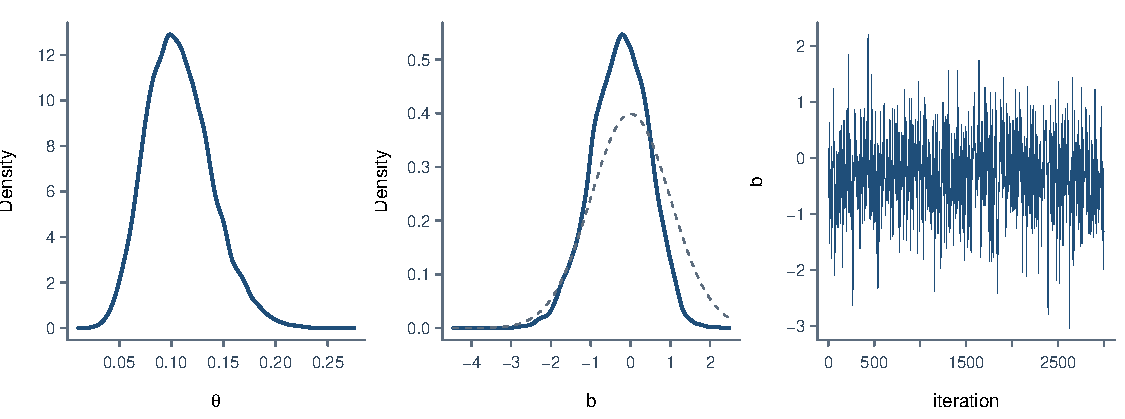
\includegraphics[width=0.98\linewidth]{ex06_posterior.pdf}\end{center}

\begin{sanity}
The posterior of $\theta$ is close to the $\dist{Beta}(11,91)$ we would get with a uniform prior (mean 0.108) --- the data dominate. The posterior of $b$ (middle panel, solid) is only slightly shifted from its $\dist N(0,1)$ prior (dashed): a single binomial count says very little about the prior's concentration.
\end{sanity}

\begin{answer}
(a) $\theta^{(0)}=0.1$, $b^{(0)}=0$. (b) $\theta\mid b,Y\sim\dist{Beta}(Y+e^b,\ n-Y+e^b)$. (c) Gibbs for $\theta$, random-walk Metropolis for $b$.
(d) $\theta$: mean 0.108, 95\% CI (0.054, 0.175); $b$: mean $-0.26$, close to its prior.
\end{answer}

\begin{takeaway}
Do not drop normalising constants that depend on the parameter you are updating --- here $\Gamma(2e^b)/\Gamma(e^b)^2$ is essential in the Metropolis ratio for $b$.
\end{takeaway}

% ================================================================= Exercise 7
\exercise{3.7 --- Shrinking clutch shooting toward each player's overall rate}

\begin{problem}{7}
Fit the following model to the NBA free throw data in the table in Exercise 22 in Chapter 1:
\[
Y_i|\theta_i\sim\dist{Binomial}(n_i,\theta_i)\quad\text{and}\quad\theta_i|m\sim\dist{Beta}[\exp(m)q_i,\exp(m)(1-q_i)],
\]
where $Y_i$ is the number of made clutch shots for player $i=1,\dots,10$, $n_i$ is the number of attempted clutch shots, $q_i\in(0,1)$ is the overall proportion, and $m\sim\dist{Normal}(0,10)$.
\begin{enumerate}[(a)]
\item Explain why this is a reasonable prior for $\theta_i$.
\item Explain the role of $m$ in the prior.
\item Derive the full conditional posterior for $\theta_1$.
\item Write your own MCMC algorithm to compute a table of posterior means and 95\% credible intervals for all 11 model parameters $(\theta_1,\dots,\theta_{10},m)$. Turn in commented code.
\item Fit the same model in JAGS. Turn in commented code, and comment on whether the two algorithms returned the same results.
\item What are the advantages and disadvantages of writing your own code as opposed to using JAGS in this problem and in general?
\end{enumerate}
\end{problem}

\begin{restate}
Instead of analysing each player alone (Chapter 1), centre each player's clutch prior on their overall free-throw percentage, and let the data decide how tightly to hold them there.
\end{restate}

\begin{recall}
For $\theta\sim\dist{Beta}(\alpha,\beta)$: $\E\theta=\frac{\alpha}{\alpha+\beta}$ and $\V\theta=\frac{\E\theta(1-\E\theta)}{\alpha+\beta+1}$. The sum $\alpha+\beta$ acts like a ``prior sample size''.
\end{recall}

\begin{keyidea}
Here $\alpha+\beta=e^m$, so $m$ is the log prior sample size: it controls how much a player's clutch rate is allowed to differ from their overall rate.
\end{keyidea}

\solution
\step{(a) Why the prior is reasonable.}
\[
\E(\theta_i\mid m)=\frac{e^mq_i}{e^mq_i+e^m(1-q_i)}=q_i.
\]
The prior is centred on the player's overall percentage --- the natural guess for their clutch percentage --- and stays inside $(0,1)$.

\step{(b) The role of $m$.}
$\V(\theta_i\mid m)=\dfrac{q_i(1-q_i)}{e^m+1}$. Large $m$: tiny variance, so $\theta_i\approx q_i$ (``clutch is the same as overall''). Small $m$: wide prior, so each player's clutch rate is estimated from their clutch data alone. Because $m$ is unknown, \emph{the data decide} how much to shrink toward $q_i$.

\step{(c) Full conditional of $\theta_1$.}
\[
p(\theta_1\mid\cdot)\propto\theta_1^{Y_1}(1-\theta_1)^{n_1-Y_1}\,\theta_1^{e^mq_1-1}(1-\theta_1)^{e^m(1-q_1)-1}
\ \Rightarrow\ \theta_1\mid\cdot\sim\dist{Beta}\big(Y_1+e^mq_1,\ n_1-Y_1+e^m(1-q_1)\big).
\]

\step{(d) The MCMC algorithm} (Gibbs for every $\theta_i$, Metropolis for $m$), from \texttt{ch03.R}:
\begin{lstlisting}
log_post_m <- function(m, theta, q) {          # log full conditional of m
  e <- exp(m)
  dnorm(m, 0, sqrt(10), log = TRUE) +          # prior N(0, variance 10)
    sum(dbeta(theta, e * q, e * (1 - q), log = TRUE))
}
for (it in seq_len(iters)) {
  e     <- exp(m)
  theta <- rbeta(10, y + e * q, n - y + e * (1 - q))     # Gibbs: all thetas at once
  cand  <- rnorm(1, m, 0.6)                              # Metropolis proposal for m
  if (log(runif(1)) < log_post_m(cand, theta, q) - log_post_m(m, theta, q)) m <- cand
  draws[it, ] <- c(theta, m)
}
\end{lstlisting}
30{,}000 iterations (2{,}000 burn-in), acceptance rate for $m$: 64\%.
\begin{center}
\small
\begin{tabular}{lccc|c}\toprule
Parameter & Posterior mean & 95\% interval & ESS & Ch.\,1 (no pooling) mean\\\midrule
$\theta$ Westbrook & 0.847 & (0.799, 0.892) & 25{,}331 & 0.844\\
$\theta$ Harden & 0.819 & (0.745, 0.859) & 953 & 0.753\\
$\theta$ Leonard & 0.878 & (0.830, 0.918) & 25{,}385 & 0.862\\
$\theta$ James & 0.678 & (0.610, 0.749) & 24{,}122 & 0.683\\
$\theta$ Thomas & 0.908 & (0.868, 0.940) & 28{,}000 & 0.894\\
$\theta$ Curry & 0.902 & (0.855, 0.947) & 18{,}438 & 0.893\\
$\theta$ Antetokounmpo & 0.753 & (0.670, 0.805) & 2{,}447 & 0.674\\
$\theta$ Wall & 0.802 & (0.751, 0.851) & 28{,}000 & 0.798\\
$\theta$ Davis & 0.788 & (0.715, 0.836) & 3{,}928 & 0.732\\
$\theta$ Durant & 0.869 & (0.801, 0.915) & 8{,}861 & 0.778\\
$m$ & 5.66 & (3.35, 9.28) & 264 & ---\\\bottomrule
\end{tabular}
\end{center}
The posterior of $m$ is large ($e^{5.66}\approx290$ pseudo-shots), so every clutch rate is pulled strongly toward the player's overall rate. Harden moves from 0.753 to 0.819, Durant (only 16 attempts) from 0.778 to 0.869.

\step{(e) JAGS.}
\begin{lstlisting}
model{
  for(i in 1:10){
    Y[i] ~ dbin(theta[i], n[i])
    theta[i] ~ dbeta(exp(m) * q[i], exp(m) * (1 - q[i]))
  }
  m ~ dnorm(0, 0.1)          # JAGS: precision 0.1 = variance 10
}
\end{lstlisting}
\JAGSexseven

\step{(f) Own code vs.\ JAGS.}
\begin{itemize}
\item \textbf{Own code} --- advantages: complete control (e.g.\ updating all $\theta_i$ in one vectorised line), often faster, and you understand every step. Disadvantages: time-consuming, easy to make algebra or coding mistakes, must tune Metropolis steps yourself.
\item \textbf{JAGS} --- advantages: you only write the model; samplers and tuning are automatic, so changing the model takes seconds. Disadvantages: a black box, can be slow or mix badly for awkward models, and limited to the distributions JAGS knows.
\end{itemize}

\begin{answer}
(a) The prior mean of $\theta_i$ is the overall rate $q_i$. (b) $e^m$ is a prior sample size controlling shrinkage toward $q_i$. (c) $\theta_1\mid\cdot\sim\dist{Beta}(Y_1+e^mq_1,\ n_1-Y_1+e^m(1-q_1))$. (d)--(e) Table above; $m\approx5.7$ means strong shrinkage; JAGS agrees. (f) Control/speed vs.\ convenience/safety.
\end{answer}

\begin{takeaway}
The data say clutch and overall shooting are very similar for most players, which is why $m$ is large. The ``clutch-choker'' effect we saw for Harden in Chapter 1 shrinks substantially once we borrow strength across players.
\end{takeaway}

% ================================================================= Exercise 8
\exercise{3.8 --- Metropolis--Hastings for a gamma shape parameter}

\begin{problem}{8}
Assume the model $Y|\theta\sim\dist{Gamma}(\theta,1)$ and prior $\theta\sim\dist{Uniform}(0,10)$. Say we observe $Y=5$. This is not a conjugate prior, and so you will use Metropolis-Hastings sampling to approximate the posterior of $\theta$.
\begin{enumerate}[(a)]
\item Plot the posterior of $\theta$ for reference, i.e. (in R),
\begin{lstlisting}
> theta <- seq(0,10,0.01)
> plot(theta,dgamma(5,theta,1),type="l")
\end{lstlisting}
\item What is a reasonable candidate distribution for $\theta$?
\item Give a formula for the acceptance probability (preferably in R code). How will you handle candidates outside $(0,10)$?
\item How will you tune the candidate distribution? Be specific.
\item Generate and plot samples from the posterior distribution, and compare results with the curve from (a)
\end{enumerate}
\end{problem}

\begin{restate}
Build, tune and check a Metropolis sampler for a one-parameter posterior that we can also draw exactly, so we can see whether the sampler works.
\end{restate}

\begin{recall}
With a uniform prior on $(0,10)$, the posterior is $p(\theta\mid Y)\propto\frac{Y^{\theta-1}e^{-Y}}{\Gamma(\theta)}$ for $0<\theta<10$ and 0 outside --- exactly the curve \texttt{dgamma(5, theta, 1)} in part (a).
\end{recall}

\begin{keyidea}
A symmetric random-walk proposal makes the acceptance ratio the plain ratio of posterior densities. Proposals outside the prior support have posterior density 0, so they are automatically rejected.
\end{keyidea}

\solution
\step{(a) Reference curve.} The red curve in the figure of part (e) is \texttt{dgamma(5, theta, 1)} rescaled to integrate to 1.

\step{(b) Candidate distribution.} A normal random walk: $\theta^*\sim\dist{Normal}(\theta^{(s-1)},\ s^2)$. It is symmetric ($q(\theta^*\mid\theta)=q(\theta\mid\theta^*)$), so the proposal densities cancel.

\step{(c) Acceptance probability.}
\[
\alpha=\min\Big\{1,\ \frac{p(\theta^*\mid Y)}{p(\theta\mid Y)}\Big\}=\min\Big\{1,\ \frac{\texttt{dgamma(5,}\theta^*\texttt{,1)}\,\mathbb 1(0<\theta^*<10)}{\texttt{dgamma(5,}\theta\texttt{,1)}}\Big\}.
\]
In R, on the log scale:
\begin{lstlisting}
log_post <- function(theta) ifelse(theta > 0 & theta < 10, dgamma(5, theta, 1, log = TRUE), -Inf)
accept   <- log(runif(1)) < log_post(cand) - log_post(theta)
\end{lstlisting}
\why{A candidate outside $(0,10)$ gets $\log p=-\infty$, so $\log R=-\infty$ and it is never accepted; the chain simply stays where it is for that iteration. Do \emph{not} just discard such candidates and redraw --- that would change the target distribution.}

\step{(d) Tuning.} Try several step sizes and look at the acceptance rate and ESS (10{,}000 iterations each):
\begin{center}
\begin{tabular}{cccc}\toprule
Step $s$ & Acceptance & ESS & Verdict\\\midrule
0.2 & 0.97 & 26 & steps too small: chain crawls\\
1.0 & 0.86 & 497 & still small\\
\textbf{2.5} & \textbf{0.65} & \textbf{1{,}725} & \textbf{best}\\
8.0 & 0.30 & 1{,}628 & many rejections\\\bottomrule
\end{tabular}
\end{center}
Rule: increase $s$ if the acceptance rate is above $\sim$50\%, decrease it if below $\sim$25\%, and pick the value with the largest ESS. We use $s=2.5$.

\step{(e) Samples.} 50{,}000 iterations (1{,}000 burn-in):
\begin{center}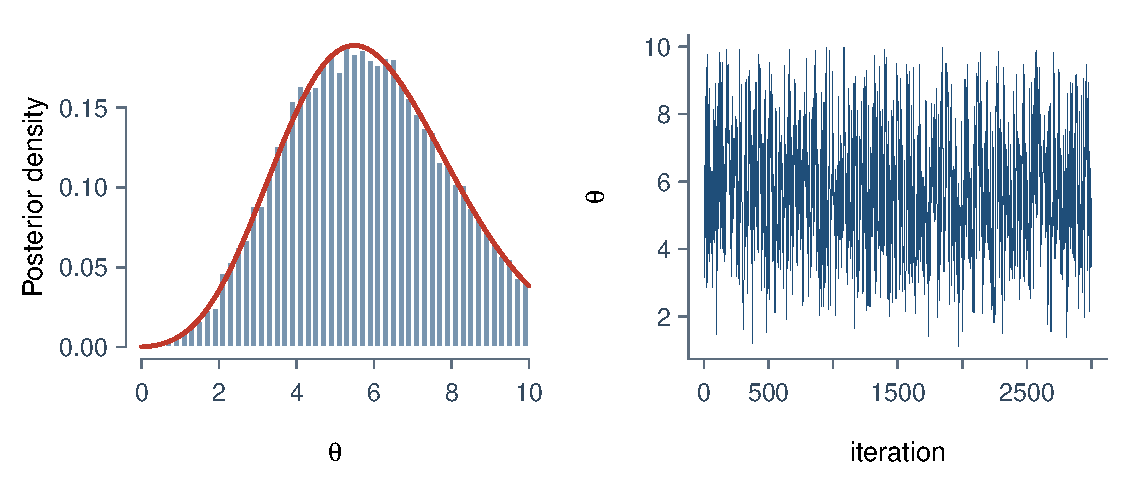
\includegraphics[width=0.98\linewidth]{ex08_metropolis.pdf}\end{center}
The histogram matches the exact curve; the trace plot looks like a hairy caterpillar.

\begin{sanity}
MCMC posterior mean 5.725 vs.\ 5.737 from the exact curve (numerical integration); 95\% interval $(2.12,\ 9.46)$.
\end{sanity}

\begin{answer}
(b) $\theta^*\sim\dist N(\theta,s^2)$. (c) $\alpha=\min\{1,\texttt{dgamma(5,cand,1)}/\texttt{dgamma(5,theta,1)}\}$, and candidates outside $(0,10)$ are rejected (chain stays put). (d) Tune $s$ by acceptance rate/ESS; $s=2.5$ works best. (e) Samples match the exact posterior (mean $\approx5.7$).
\end{answer}

\begin{takeaway}
A very high acceptance rate is \emph{not} good: it usually means the steps are tiny and the chain barely moves (ESS 26 at 97\% acceptance!).
\end{takeaway}

% ================================================================= Exercise 9
\exercise{3.9 --- A Student-$t$ model for the galaxies data}

\begin{problem}{9}
Open and plot the galaxies data in R using the code below,
\begin{lstlisting}
> library(MASS)
> data(galaxies)
> ?galaxies
> Y <- galaxies
> n <- length(Y)
> hist(Y,breaks=25)
\end{lstlisting}
Model the observations $Y_1,\dots,Y_{82}$ using the Student's t-distribution with location $\mu$, scale $\sigma$ and degrees of freedom $k$. Assume prior distributions $\mu\sim\dist{Normal}(0,10000^2)$, $1/\sigma^2=\tau\sim\dist{Gamma}(0.01,0.01)$ and $k\sim\dist{Uniform}(1,30)$.
\begin{enumerate}[(a)]
\item Give reasonable initial values for each of the three parameters.
\item Fit the model using JAGS. Report trace plots of each parameter, and discuss convergence.
\item Graphically compare the t distribution with parameters set to their posterior mean with the observed data. Does the model fit the data well?
\end{enumerate}
\end{problem}

\begin{restate}
Fit a heavy-tailed bell curve to the velocities of 82 galaxies, check that the sampler converged, and see whether a single bell curve describes the data.
\end{restate}

\begin{recall}
\textbf{The $t$ distribution as a scale mixture.} If $\lambda_i\sim\dist{Gamma}(k/2,k/2)$ and $Y_i\mid\lambda_i\sim\dist{Normal}(\mu,\sigma^2/\lambda_i)$, then marginally $Y_i\sim t_k(\mu,\sigma)$. Small $\lambda_i$ = an observation allowed to be far out. This makes almost every full conditional standard.
\end{recall}

\begin{keyidea}
Use the data to pick initial values (centre and spread). With the latent $\lambda_i$, the full conditionals are: $\mu$ normal, $\tau$ gamma, $\lambda_i$ gamma; $k$ needs a Metropolis step.
\end{keyidea}

\solution
\step{(a) Initial values.} $\mu^{(0)}=$ median of the data $=20{,}834$; $\tau^{(0)}=1/\text{var}(Y)$ (so $\sigma^{(0)}\approx4{,}600$); $k^{(0)}=5$ (moderately heavy tails). For a convergence check we also start chains far away: $(\mu,\sigma,k)=(15{,}000,\ 5{,}000,\ 25)$ and $(25{,}000,\ 1{,}000,\ 3)$.

\step{(b) Full conditionals used by our sampler.}
\[
\mu\mid\cdot\sim\dist N\Big(\frac{\tau\sum\lambda_iY_i}{\tau\sum\lambda_i+10^{-8}},\ \frac{1}{\tau\sum\lambda_i+10^{-8}}\Big),\quad
\tau\mid\cdot\sim\dist{Gamma}\Big(0.01+\frac n2,\ 0.01+\frac{\sum\lambda_i(Y_i-\mu)^2}{2}\Big),
\]
\[
\lambda_i\mid\cdot\sim\dist{Gamma}\Big(\frac{k+1}{2},\ \frac{k+\tau(Y_i-\mu)^2}{2}\Big),\qquad k:\ \text{Metropolis step on }(1,30).
\]
\step{(b) Trace plots} (two chains from the extreme starting values, 20{,}000 iterations each):
\begin{center}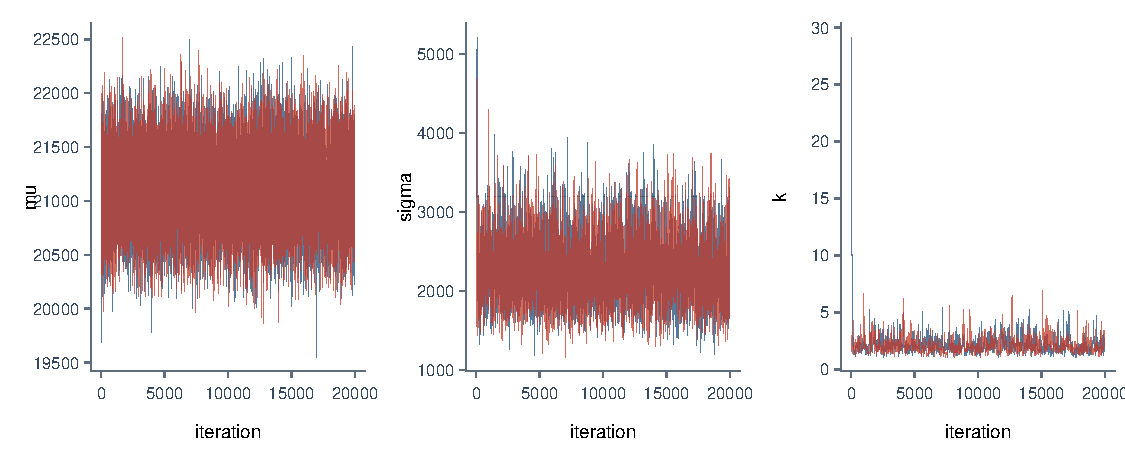
\includegraphics[width=0.98\linewidth]{ex09_traces.pdf}\end{center}
Both chains forget their starting values within a few hundred iterations and then overlap. $\hat R=1.000$ for all three parameters; ESS: $\mu$ 13{,}284, $\sigma$ 1{,}131, $k$ 494 (after 2{,}000 burn-in per chain). $k$ mixes slowest, as is typical for degrees of freedom, but all ESS are adequate.
\begin{center}
\begin{tabular}{lccc}\toprule
 & Mean & SD & 95\% interval\\\midrule
$\mu$ & 21{,}115 & 325 & (20{,}481, 21{,}757)\\
$\sigma$ & 2{,}240 & 349 & (1{,}641, 3{,}008)\\
$k$ & 2.1 & 0.6 & (1.2, 3.6)\\\bottomrule
\end{tabular}
\end{center}
JAGS (\texttt{Y[i] \textasciitilde{} dt(mu, tau, k)}):
\JAGSexnine

\step{(c) Fit.}
\begin{center}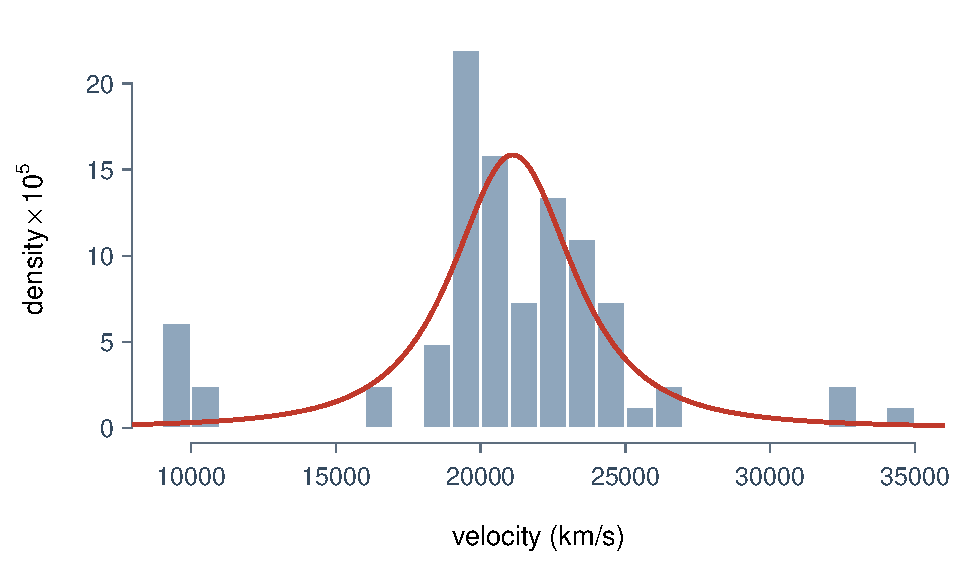
\includegraphics[width=0.72\linewidth]{ex09_fit.pdf}\end{center}
\textbf{The fit is poor.} The histogram has several clusters (around 10{,}000, 20{,}000--23{,}000 and 33{,}000 km/s); a single symmetric $t$ curve cannot reproduce multiple peaks. The model ``explains'' the outer clusters by choosing very heavy tails ($k\approx2$).

\begin{answer}
(a) $\mu^{(0)}=\text{median}(Y)$, $\tau^{(0)}=1/\text{var}(Y)$, $k^{(0)}=5$. (b) Converged ($\hat R=1.00$, adequate ESS); $\mu\approx21{,}100$, $\sigma\approx2{,}240$, $k\approx2.1$. (c) Poor fit: the data are multi-modal and a single $t$ density cannot capture the clusters --- a mixture model is needed.
\end{answer}

\begin{takeaway}
Convergence of the sampler tells you nothing about whether the \emph{model} is right. Always compare the fitted model with the data.
\end{takeaway}

% ================================================================= Exercise 10
\exercise{3.10 --- A Laplace model for the galaxies data, on a grid}

\begin{problem}{10}
Download the galaxy data
\begin{lstlisting}
> library(MASS)
> data(galaxies)
> Y <- galaxies
\end{lstlisting}
Suppose $Y_i|\theta\iid\dist{Laplace}(\mu,\sigma)$ for $i=1,\dots,n$ where $\theta=(\mu,\sigma)$.
\begin{enumerate}[(a)]
\item Assuming the improper prior $\sigma\sim\dist{Uniform}(0,100000)$ and $\pi(\mu)=1$ for all $\mu\in(-\infty,\infty)$, plot the joint posterior distribution of $\theta$ and the marginal posterior distributions of $\mu$ and $\sigma$.
\item Compute the posterior mean of $\theta$ from your analysis in (a), and plot the Laplace PDF with these values against the observed data. Does the model fit the data well?
\item Plot the posterior predictive distribution (PPD) for a new observation $Y^*|\theta\sim\dist{Laplace}(\mu,\sigma)$. How do the mean and variance of the PPD compare to the mean and variance of the ``plug-in'' distribution from (b)?
\end{enumerate}
\end{problem}

\begin{restate}
Fit a double-exponential (Laplace) curve with two unknowns by brute force on a 2-D grid, check the fit, and compare predicting with uncertainty vs.\ plugging in estimates.
\end{restate}

\begin{recall}
$\dist{Laplace}(\mu,\sigma)$: density $\frac{1}{2\sigma}\exp\{-|y-\mu|/\sigma\}$, mean $\mu$, variance $2\sigma^2$. A Laplace draw is $\mu+\sigma(E_1-E_2)$ with $E_1,E_2\iid\dist{Exponential}(1)$.
\end{recall}

\begin{keyidea}
With two parameters, \textbf{grid approximation} is easy and exact enough: evaluate the log posterior on a $300\times300$ grid of $(\mu,\sigma)$, exponentiate, normalise, and sum over rows/columns for the marginals.
\end{keyidea}

\solution
\step{(a) Step 1 --- the log posterior.}
With flat priors (the upper bound 100{,}000 is far from where the likelihood lives),
\[
\log p(\mu,\sigma\mid\mathbf Y)=-n\log\sigma-\frac{1}{\sigma}\sum_{i=1}^n|Y_i-\mu|+\text{const}.
\]
\step{(a) Step 2 --- evaluate on a grid.} $\mu\in[19{,}000,\ 23{,}000]$ and $\sigma\in[2{,}000,\ 5{,}500]$, 300 points each. Subtract the maximum before exponentiating (avoids underflow), divide by the total, then sum over $\sigma$ (for $\mu$) and over $\mu$ (for $\sigma$).
\begin{center}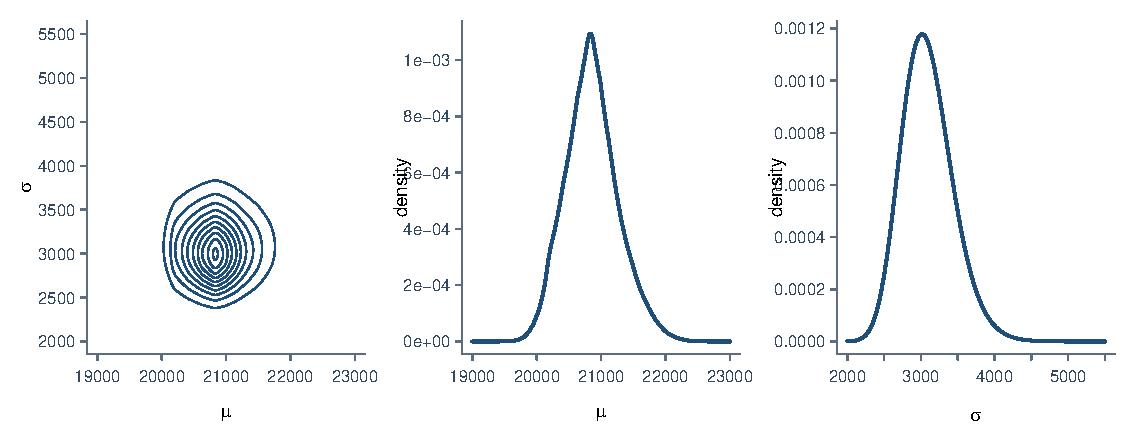
\includegraphics[width=0.98\linewidth]{ex10_posterior.pdf}\end{center}
Left: joint posterior contours. The $\mu$ marginal is flat-topped/irregular because the Laplace likelihood is piecewise linear in $\mu$ (the posterior mode is the sample median).

\step{(b) Posterior means and fit.}
$\E(\mu\mid\mathbf Y)=20{,}856$ (sample median 20{,}834) and $\E(\sigma\mid\mathbf Y)=3{,}091$.
\begin{center}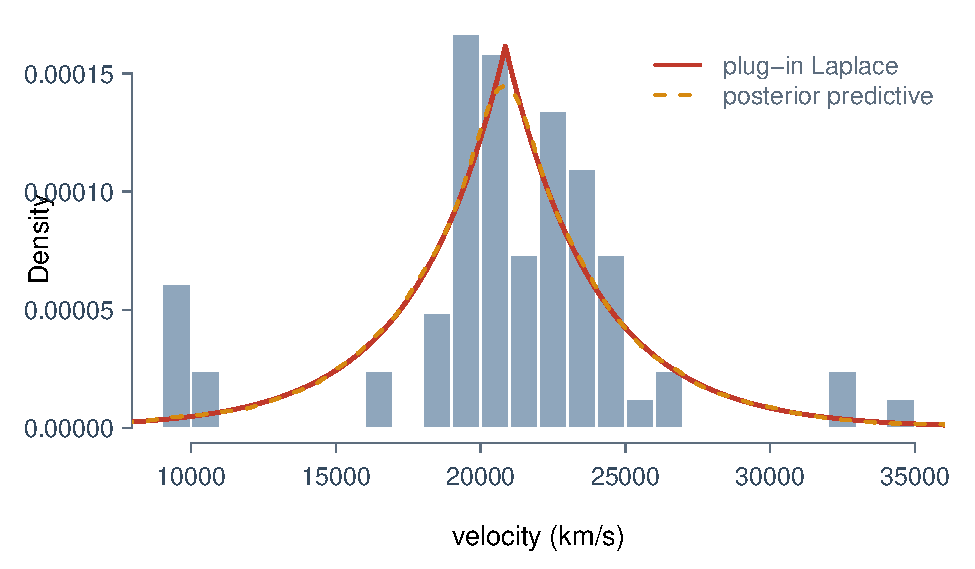
\includegraphics[width=0.72\linewidth]{ex10_fit.pdf}\end{center}
\textbf{Not a good fit}, for the same reason as Exercise 9: the data have several clusters and the Laplace density has a single sharp peak.

\step{(c) Posterior predictive.}
Draw $10^5$ grid cells with probability equal to their posterior mass, then draw $Y^*\sim\dist{Laplace}(\mu,\sigma)$ for each.
\begin{center}
\begin{tabular}{lcc}\toprule
 & Mean & Variance\\\midrule
Plug-in $\dist{Laplace}(20{,}856,\ 3{,}091)$ & 20{,}856 & $2\hat\sigma^2=1.911\times10^7$\\
Posterior predictive & 20{,}840 & $1.937\times10^7$\\\bottomrule
\end{tabular}
\end{center}
\why{By the laws of total expectation and variance: $\E(Y^*)=\E(\mu)$, so the means agree; $\V(Y^*)=\E(2\sigma^2)+\V(\mu)>2[\E\sigma]^2$, so the PPD is wider --- here by only about 1\%, because with $n=82$ the parameters are well determined.}

\begin{answer}
(a) See the contour and marginal plots. (b) $\hat\mu\approx20{,}856$, $\hat\sigma\approx3{,}091$; the Laplace fits poorly (multi-modal data). (c) Same mean; the PPD variance is about 1.3\% larger than the plug-in variance, because it also accounts for uncertainty in $(\mu,\sigma)$.
\end{answer}

\begin{takeaway}
The PPD is always at least as spread out as the plug-in distribution. The difference matters for small samples and disappears as $n$ grows.
\end{takeaway}

% ================================================================= Exercise 11
\exercise{3.11 --- Reggie Jackson with MCMC diagnostics}

\begin{problem}{11}
In Section 2.5 we compared Reggie Jackson's home run rate in the regular season and World Series. He hit 563 home runs in 2820 regular-season games and 10 home runs in 27 World Series games (a player can hit 0, 1, 2, \dots{} home runs in a game). Assuming Uniform(0,10) priors for both home run rates, use JAGS to summarize the posterior distribution of (i) his home run rate in the regular season, (ii) his home run rate in the World Series, and (iii) the ratio of these rates. Provide trace plots for all three parameters and discuss convergence of the MCMC sampler including appropriate convergence diagnostics.
\end{problem}

\begin{restate}
Redo Exercise 2.2 with uniform priors and MCMC, and show how to check that the sampler has converged.
\end{restate}

\begin{keyidea}
A derived quantity (the ratio) is free in MCMC: compute it from each pair of draws. Check convergence with several chains from very different starting values.
\end{keyidea}

\solution
\step{Model.} $Y_R\mid\lambda_R\sim\dist{Poisson}(2820\lambda_R)$, $Y_{WS}\mid\lambda_{WS}\sim\dist{Poisson}(27\lambda_{WS})$, $\lambda_R,\lambda_{WS}\iid\dist{Uniform}(0,10)$. Exact posteriors: $\dist{Gamma}(564,2820)$ and $\dist{Gamma}(11,27)$ (truncated at 10, negligibly).
\begin{lstlisting}
model{
  Y_reg ~ dpois(N_reg * lambda_reg);   Y_ws ~ dpois(N_ws * lambda_ws)
  lambda_reg ~ dunif(0, 10);           lambda_ws ~ dunif(0, 10)
  ratio <- lambda_ws / lambda_reg
}
\end{lstlisting}
\step{Our own sampler.} Random-walk Metropolis on $\log\lambda$ (with the Jacobian term), two chains started at 0.05 and 2 HR/game, 20{,}000 iterations, 2{,}000 burn-in.
\begin{center}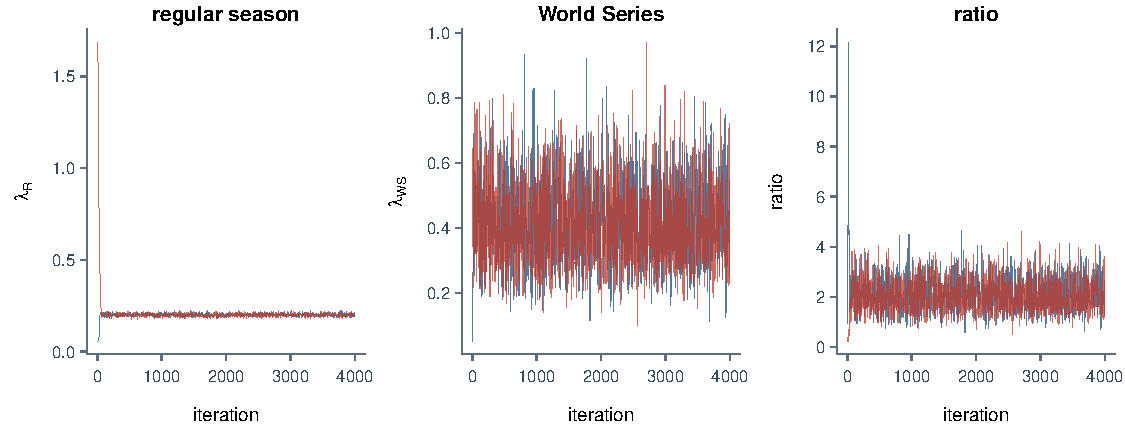
\includegraphics[width=0.98\linewidth]{ex11_traces.pdf}\end{center}
\begin{center}
\begin{tabular}{lcccccc}\toprule
 & Mean & SD & 95\% interval & $\hat R$ & ESS & Exact mean\\\midrule
$\lambda_R$ & 0.200 & 0.008 & (0.184, 0.217) & 1.000 & 8{,}213 & 564/2820 = 0.200\\
$\lambda_{WS}$ & 0.409 & 0.123 & (0.208, 0.682) & 1.000 & 8{,}596 & 11/27 = 0.407\\
ratio & 2.05 & 0.62 & (1.04, 3.42) & 1.000 & 8{,}607 & ---\\\bottomrule
\end{tabular}
\end{center}
$\Prob(\lambda_{WS}>\lambda_R\mid\text{data})=0.98$.
\step{JAGS.}
\JAGSexeleven

\step{Convergence discussion.}
\begin{itemize}
\item \textbf{Trace plots}: both chains move quickly from their (deliberately bad) starts into the same region and overlap thereafter.
\item \textbf{Gelman--Rubin}: $\hat R=1.000$ for all three quantities (threshold 1.1).
\item \textbf{ESS}: over 8{,}000 for each, far more than needed for means and 95\% intervals.
\item \textbf{Exact check}: MCMC means match the exact Gamma posterior means.
\end{itemize}

\begin{answer}
(i) $\lambda_R$: mean 0.200, 95\% CI (0.184, 0.217). (ii) $\lambda_{WS}$: mean 0.41, 95\% CI (0.21, 0.68). (iii) Ratio: mean 2.05, 95\% CI (1.04, 3.42), $\Prob(\text{ratio}>1)=0.98$. The sampler has clearly converged.
\end{answer}

\begin{takeaway}
Compare with Exercise 2.2: the $\dist{Uniform}(0,10)$ prior (equivalent to $\dist{Gamma}(1,0)$, one ``pseudo home run'') pulls the World Series rate up from 0.37 to 0.41, making the ratio interval exclude 1. With only 10 home runs, the prior matters.
\end{takeaway}

% ================================================================= Exercise 12
\exercise{3.12 --- Is the discovery rate of bivalve species changing?}

\begin{problem}{12}
As discussed in Section 1.6, [47] report that the number of marine bivalve species discovered each year from 2010-2015 was 64, 13, 33, 18, 30 and 20. Denote $Y_t$ as the number of species discovered in year $2009+t$ (so that $Y_1=64$ is the count for 2010). Use JAGS to fit the model
\[
Y_t|\alpha,\beta\overset{indep}{\sim}\dist{Poisson}(\lambda_t)
\]
where $\lambda_t=\exp(\alpha+\beta t)$ and $\alpha,\beta\sim\dist{Normal}(0,10^2)$. Summarize the posterior of $\alpha$ and $\beta$ and verify that the MCMC sampler has converged. Does this analysis provide evidence that the rate of discovery is changing over time?
\end{problem}

\begin{restate}
Fit a Poisson regression with a log-linear time trend to six yearly counts and decide whether the trend slope $\beta$ is non-zero.
\end{restate}

\begin{recall}
In $\lambda_t=e^{\alpha+\beta t}$, $e^{\beta}$ is the \emph{multiplicative} change in the expected count per year: $\beta=-0.18$ means $e^{-0.18}=0.835$, a 16.5\% decrease per year.
\end{recall}

\begin{keyidea}
The log posterior is easy to write: $\sum_t\big[Y_t(\alpha+\beta t)-e^{\alpha+\beta t}\big]+\log\pi(\alpha)+\log\pi(\beta)$. Neither full conditional is standard, so use Metropolis (Exercise 13) or JAGS.
\end{keyidea}

\solution
\step{JAGS model.}
\begin{lstlisting}
model{
  for(t in 1:6){
    Y[t] ~ dpois(lambda[t])
    log(lambda[t]) <- alpha + beta * t
  }
  alpha ~ dnorm(0, 0.01)       # precision 0.01 = variance 10^2
  beta  ~ dnorm(0, 0.01)
}
\end{lstlisting}
\JAGSextwelve

\step{Posterior summary} (our Metropolis sampler from Exercise 13; three chains $\times$ 27{,}000 kept draws):
\begin{center}
\begin{tabular}{lcccccc}\toprule
 & Mean & SD & 95\% interval & $\hat R$ & ESS\\\midrule
$\alpha$ & 3.969 & 0.156 & (3.657, 4.268) & 1.000 & 1{,}994\\
$\beta$ & $-0.181$ & 0.046 & $(-0.270,\ -0.093)$ & 1.001 & 2{,}046\\\bottomrule
\end{tabular}
\end{center}
\step{Convergence.} Three chains from very different starting points ($(0,0)$, $(5,-1)$, $(2,1)$) overlap after a short burn-in (trace plots in Exercise 13); $\hat R\le1.001$ and ESS around 2{,}000 for both parameters.

\step{Is the rate changing?}
$\Prob(\beta<0\mid\mathbf Y)>0.9999$ and the 95\% interval for $\beta$ excludes 0. The posterior median yearly change is $e^{-0.18}-1=-16.5\%$.

\begin{sanity}
The classical Poisson GLM gives $\hat\alpha=3.976$, $\hat\beta=-0.181$ --- the same as the posterior means, as expected with vague priors.
\end{sanity}

\begin{answer}
$\alpha$: mean 3.97 (3.66, 4.27); $\beta$: mean $-0.181$ $(-0.270,-0.093)$. Converged ($\hat R\approx1$). Yes --- strong evidence of a decreasing discovery rate, about 16\% fewer discoveries per year.
\end{answer}

\begin{takeaway}
Caution: the count of 64 in 2010 is a big outlier and the counts are over-dispersed (Chapter 1, Exercise 16). A Poisson model then gives over-confident intervals; a negative binomial model would be more honest and the evidence would be weaker.
\end{takeaway}

% ================================================================= Exercise 13
\exercise{3.13 --- Writing the Metropolis sampler by hand}

\begin{problem}{13}
Write your own Metropolis sampler (i.e., not JAGS) for the previous problem. Turn in commented code, report your candidate distribution for each parameters and corresponding acceptance ratio, and use trace plots for each parameter to show the chains have converged.
\end{problem}

\begin{restate}
Implement the sampler for Exercise 12 yourself and show it works.
\end{restate}

\begin{keyidea}
One-parameter-at-a-time random-walk Metropolis: propose a change to $\alpha$ only, accept/reject; then the same for $\beta$. Tune each step size separately.
\end{keyidea}

\solution
\step{Commented code} (from \texttt{ch03.R}):
\begin{lstlisting}
y <- c(64, 13, 33, 18, 30, 20); t <- 1:6
log_post <- function(ab) {                       # log posterior up to a constant
  eta <- ab[1] + ab[2] * t                       # log(lambda_t)
  sum(y * eta - exp(eta)) +                      # Poisson log-likelihood
    sum(dnorm(ab, 0, 10, log = TRUE))            # N(0, 10^2) priors
}
metro <- function(start, steps = c(0.12, 0.035), iters = 30000) {
  ab <- start; lp <- log_post(ab)
  for (it in seq_len(iters)) {
    for (j in 1:2) {                             # update alpha, then beta
      cand <- ab; cand[j] <- rnorm(1, ab[j], steps[j])   # normal random walk
      lp_cand <- log_post(cand)
      if (log(runif(1)) < lp_cand - lp) { ab <- cand; lp <- lp_cand }   # accept
    }
    draws[it, ] <- ab
  }
}
\end{lstlisting}
\step{Candidate distributions and acceptance.}
$\alpha^*\sim\dist{Normal}(\alpha,\ 0.12^2)$ and $\beta^*\sim\dist{Normal}(\beta,\ 0.035^2)$, chosen by trial and error. Acceptance rates: $\alpha$ 57\%, $\beta$ 57\%.
\step{Trace plots} (three chains, the first 6{,}000 iterations, plus the posterior of $\beta$):
\begin{center}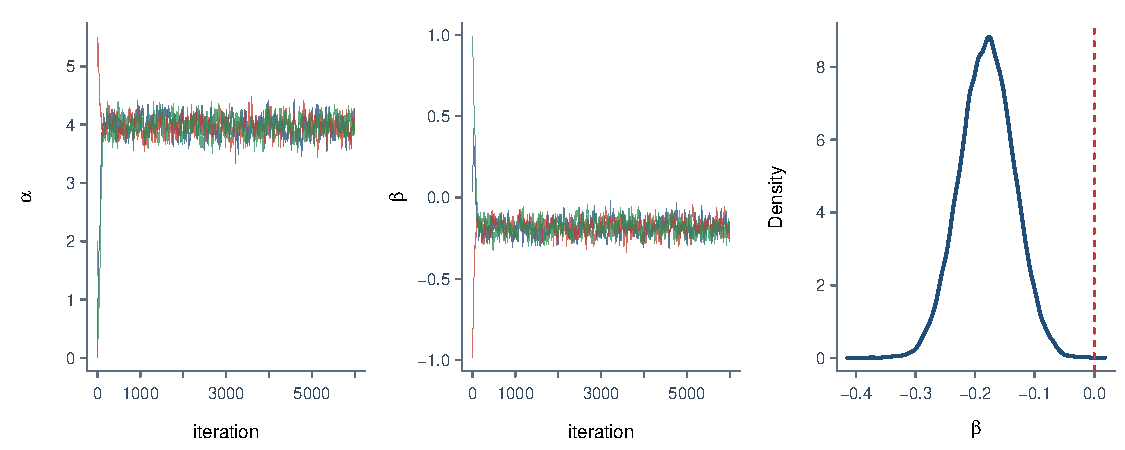
\includegraphics[width=0.98\linewidth]{ex12_traces.pdf}\end{center}

\begin{sanity}
$\hat R=1.0004$ ($\alpha$) and $1.0005$ ($\beta$); the posterior means agree with JAGS and with the GLM.
\end{sanity}

\begin{answer}
Normal random-walk candidates with SD 0.12 ($\alpha$) and 0.035 ($\beta$); acceptance $\approx57\%$ each; trace plots and $\hat R\approx1$ show convergence. Results as in Exercise 12.
\end{answer}

\begin{takeaway}
The posterior correlation between $\alpha$ and $\beta$ is $-0.88$, which slows a one-at-a-time sampler (ESS only $\approx2{,}000$ out of 81{,}000). Centring time ($t-3.5$ instead of $t$) would make $\alpha$ and $\beta$ nearly uncorrelated and the sampler far more efficient.
\end{takeaway}

% ================================================================= Exercise 14
\exercise{3.14 --- Which dose is best?}

\begin{problem}{14}
A clinical trial assigned 100 patients each to the placebo, the low dose of a new drug, and the high dose of the new drug (for a total of 300 patients); the data are given in the table below.
\begin{center}
\begin{tabular}{lcc}\toprule
Treatment & Positive outcome & Negative outcome\\\midrule
Placebo & 52 & 48\\
Low dose & 60 & 40\\
High dose & 54 & 46\\\bottomrule
\end{tabular}
\end{center}
Conduct a Bayesian analysis using JAGS with uniform priors on the probability of a patient having a positive outcome under each treatment.
\begin{enumerate}[(a)]
\item Report the posterior mean and 95\% interval for the probability of a positive outcome for each treatment group.
\item Compute the posterior probability that the low dose is the best of the three treatment options.
\end{enumerate}
\end{problem}

\begin{restate}
Three independent success rates; estimate each and the probability that the low dose has the highest rate.
\end{restate}

\begin{keyidea}
Each arm is a beta--binomial: $p_j\mid Y_j\sim\dist{Beta}(1+Y_j,\ 1+100-Y_j)$. ``Low dose is best'' is the event $\{p_2>p_1\text{ and }p_2>p_3\}$; its probability is the fraction of joint posterior draws in which it happens.
\end{keyidea}

\solution
\step{JAGS model.}
\begin{lstlisting}
model{
  for(j in 1:3){
    Y[j] ~ dbin(p[j], 100)
    p[j] ~ dunif(0, 1)
  }
  low_best <- step(p[2] - p[1]) * step(p[2] - p[3])   # 1 if low dose is best
}
\end{lstlisting}
\JAGSexfourteen
\step{(a) Posteriors} ($10^6$ exact draws from each Beta posterior):
\begin{center}
\begin{tabular}{lccc}\toprule
Arm & Posterior & Mean & 95\% interval\\\midrule
Placebo & $\dist{Beta}(53,49)$ & 0.520 & (0.423, 0.615)\\
Low dose & $\dist{Beta}(61,41)$ & 0.598 & (0.502, 0.691)\\
High dose & $\dist{Beta}(55,47)$ & 0.539 & (0.442, 0.635)\\\bottomrule
\end{tabular}
\end{center}
\step{(b) Probability each arm is best.} For each joint draw $(p_1,p_2,p_3)$, record which is largest:
\[
\Prob(\text{placebo best})=0.093,\qquad\Prob(\textbf{low dose best})=\mathbf{0.737},\qquad\Prob(\text{high dose best})=0.170.
\]

\begin{answer}
(a) Placebo 0.520 (0.42, 0.62); low dose 0.598 (0.50, 0.69); high dose 0.539 (0.44, 0.63). \quad (b) $\Prob(\text{low dose best}\mid\text{data})\approx0.74$.
\end{answer}

\begin{takeaway}
The intervals overlap a lot, so 74\% is suggestive but far from conclusive. The ranking probability is a quantity that is very natural in Bayesian analysis but awkward to obtain from classical tests.
\end{takeaway}

% ================================================================= Exercise 15
\exercise{3.15 --- A normal mixture with vague but proper priors}

\begin{problem}{15}
Consider the normal mixture model
\[
Y_i|\theta\iid f(y|\theta)=\frac12[\phi(y-\theta)+\phi(y)],
\]
for $i=1,\dots,n$ where $\theta\in\mathbb R$ and $\phi(z)=\exp\{-z^2/2\}/\sqrt{2\pi}$ denotes the density of a standard normal distribution. We have shown (Section 2.4, problem 14) that an improper prior cannot be used for this likelihood. In this problem we explore the use of vague but proper priors. Analyze data simulated in R as:
\begin{lstlisting}
> set.seed(27695)
> theta_true <- 4
> n          <- 30
> B          <- rbinom(n,1,0.5)
> Y          <- rnorm(n,B*theta_true,1)
\end{lstlisting}
\begin{enumerate}[(a)]
\item Argue that the R code above generates samples from $f(y|\theta)$.
\item Plot the simulated data, and plot $f(y|\theta)$ for $y\in[-3,10]$ separately for $\theta=\{2,4,6\}$.
\item Assuming prior $\theta\sim\dist{Normal}(0,10^2)$, obtain the MAP estimate of $\theta$ and its asymptotic posterior standard deviation using the following R code:
\begin{lstlisting}
> nlp <- function(theta,Y){
>   like <- 0.5*dnorm(Y,0,1)+
>           0.5*dnorm(Y,theta,1)
>   prior <- dnorm(theta,0,10)
>   neg_log_post <- -sum(log(like))-sum(log(prior))
> return(neg_log_post)}
> map     <- optim(mean(Y),nlp,Y=Y,hessian=TRUE)
> map_est <- map$par
> map_sd  <- 1/sqrt(map$hessian)
\end{lstlisting}
\item Suppose the prior distribution is $\theta\sim N(0,10^k)$. Plot the posterior density of $\theta$ for $k\in\{0,1,2,3\}$, and compare these posterior densities with the asymptotic normal distribution in (c) (by overlaying all five densities on the same plot).
\item Use JAGS to fit this model via its mixture representation $Y_i|B_i,\theta\sim\dist{Normal}(B_i\theta,1)$, where $B_i\iid\dist{Bernoulli}(0.5)$ and $\theta\sim\dist{Normal}(0,10^2)$. Compare the posterior distribution of $\theta$ with the results from part (d).
\end{enumerate}
\end{problem}

\begin{restate}
Half the data are $\dist N(0,1)$ noise, half are centred at the unknown $\theta$. Estimate $\theta$ three ways --- MAP + normal approximation, exact grid posterior for several priors, and a latent-variable Gibbs sampler --- and compare.
\end{restate}

\begin{recall}
\textbf{Law of total probability for densities}: if $B\sim\dist{Bernoulli}(0.5)$ and $Y\mid B\sim\dist N(B\theta,1)$, then $f(y)=0.5\,\phi(y)+0.5\,\phi(y-\theta)$.
\end{recall}

\begin{keyidea}
Adding the latent labels $B_i$ makes the model easy: given the labels, $\theta$ is a normal mean estimated from the $B_i=1$ observations only.
\end{keyidea}

\solution
\step{(a) Why the code samples from $f$.} For each $i$, \texttt{rbinom} flips a fair coin $B_i$; then \texttt{rnorm(n, B*theta, 1)} draws from $\dist N(0,1)$ if $B_i=0$ and from $\dist N(\theta,1)$ if $B_i=1$. Averaging over the coin (Recall box), the density of $Y_i$ is $\frac12\phi(y)+\frac12\phi(y-\theta)=f(y\mid\theta)$.

\step{(b) Data and densities.}
\begin{center}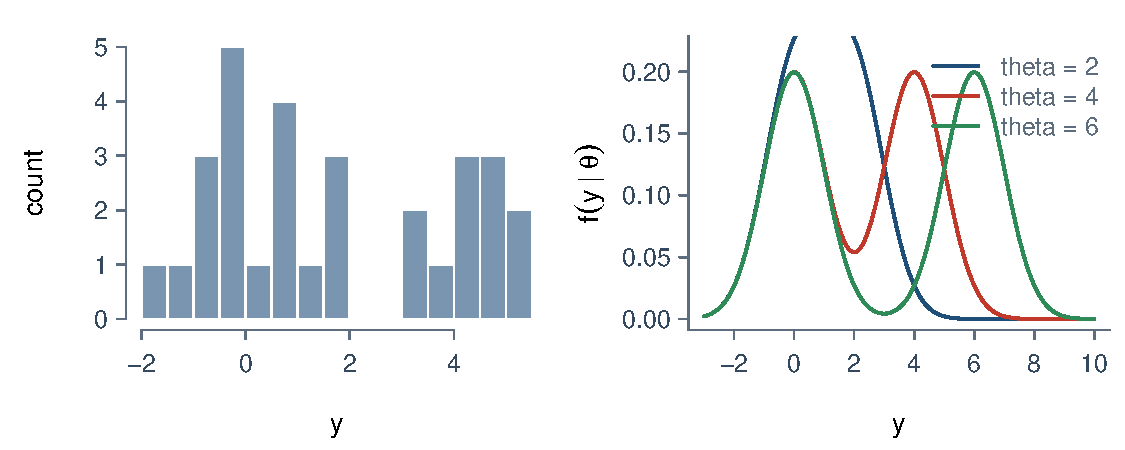
\includegraphics[width=0.98\linewidth]{ex15_data.pdf}\end{center}
The data show two bumps (near 0 and near 4). For $\theta=2$ the two components overlap into one lumpy bump; for $\theta=4,6$ they separate.

\step{(c) MAP and asymptotic SD.} Running the given code: $\hat\theta_{MAP}=\mathbf{4.179}$ and asymptotic SD $=\mathbf{0.339}$, i.e.\ $\theta\mid\mathbf Y\approx\dist N(4.179,\ 0.339^2)$.

\step{(d) Exact posteriors for four priors} (grid of 4{,}001 values; prior variance $10^k$):
\begin{center}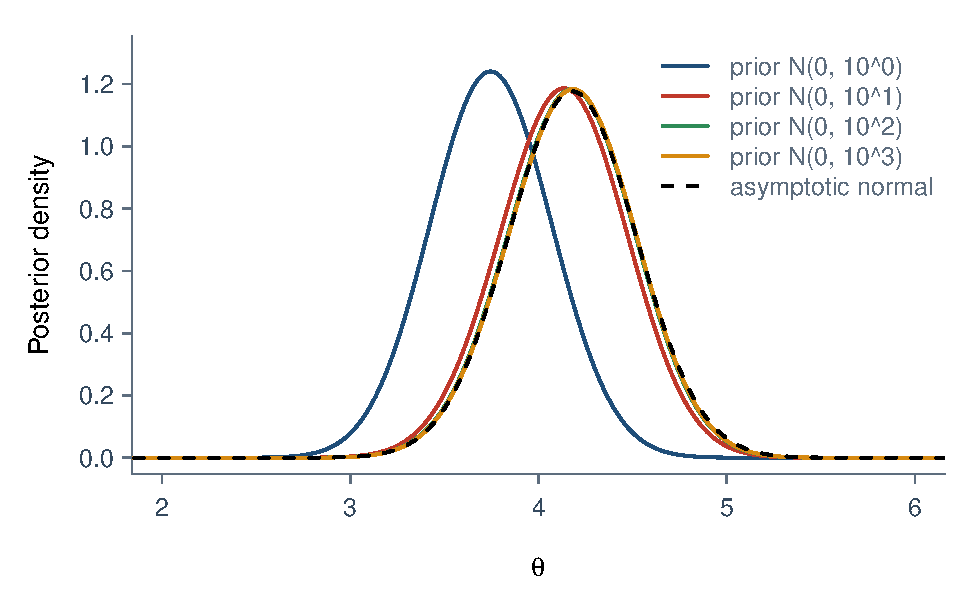
\includegraphics[width=0.72\linewidth]{ex15_posteriors.pdf}\end{center}
\begin{center}
\begin{tabular}{ccc}\toprule
Prior & Posterior mean & Posterior SD\\\midrule
$\dist N(0,10^0)$ & 3.749 & 0.320\\
$\dist N(0,10^1)$ & 4.129 & 0.334\\
$\dist N(0,10^2)$ & 4.171 & 0.335\\
$\dist N(0,10^3)$ & 4.175 & 0.335\\
asymptotic normal (c) & 4.179 & 0.339\\\bottomrule
\end{tabular}
\end{center}
Only the tight $\dist N(0,1)$ prior (SD 1, which considers $\theta=4$ very unlikely) pulls the posterior noticeably toward 0. For $k\ge1$ all posteriors nearly coincide with each other and with the normal approximation.

\step{(e) Latent-variable sampler.}
Gibbs updates: $B_i\mid\theta,Y_i\sim\dist{Bernoulli}\Big(\frac{\phi(Y_i-\theta)}{\phi(Y_i)+\phi(Y_i-\theta)}\Big)$, and $\theta\mid\mathbf B,\mathbf Y\sim\dist N\Big(\frac{\sum_{B_i=1}Y_i}{n_1+0.01},\ \frac{1}{n_1+0.01}\Big)$ where $n_1=\sum B_i$.
Our Gibbs sampler gives mean 4.177, SD 0.337 --- matching the $k=2$ grid posterior. JAGS:
\JAGSexfifteen

\begin{answer}
(a) Coin flip, then the chosen normal: the marginal is the mixture. (b) See plots. (c) MAP 4.179, SD 0.339. (d) For prior variance $\ge10$ the posterior is $\approx\dist N(4.17,0.335^2)$; the $\dist N(0,1)$ prior shrinks it to 3.75. (e) The latent-variable MCMC reproduces the $k=2$ posterior.
\end{answer}

\begin{takeaway}
A \emph{proper} prior fixes the impropriety problem of Exercise 2.17, and here any reasonably vague proper prior gives the same answer --- because the data do contain information about $\theta$. The impropriety only bites in the far tails.
\end{takeaway}

% ================================================================= Exercise 16
\exercise{3.16 --- The shifted exponential distribution}

\begin{problem}{16}
Let $Y_1,\dots,Y_n$ be a random sample from a shifted exponential distribution with density
\[
f(y|\alpha,\beta)=\begin{cases}\beta\exp^{-\beta(y-\alpha)} & y\ge\alpha\\ 0 & y<\alpha\end{cases}
\]
where $\alpha>0$ and $\beta>0$ are the parameters of interest. Assume prior distributions $\alpha\sim\dist{Uniform}(0,c)$ and $\beta\sim\dist{Gamma}(a,b)$.
\begin{enumerate}[(a)]
\item Plot $f(y|\alpha,\beta)$ for $\alpha=2$ and $\beta=3$ and $y\in[0,5]$, give interpretations of $\alpha$ and $\beta$, and describe a real experiment where this model might be appropriate.
\item Give the full conditional distributions of $\alpha$ and $\beta$, and determine if they are members of a common family of distributions.
\item Write pseudo code for an MCMC sampler including initial values, full details of each sampling step, and how you plan to assess convergence.
\end{enumerate}
\end{problem}

\begin{restate}
A waiting time that cannot be shorter than $\alpha$ and then decays exponentially at rate $\beta$. Interpret it, derive the Gibbs updates, and write the algorithm.
\end{restate}

\begin{recall}
\textbf{Indicator functions.} The density is $\beta e^{-\beta(y-\alpha)}\mathbb 1(y\ge\alpha)$. For a whole sample, $\prod_i\mathbb 1(Y_i\ge\alpha)=\mathbb 1(\alpha\le\min_iY_i)$: the threshold can be at most the smallest observation.
\end{recall}

\begin{keyidea}
The full conditional of $\alpha$ lives on a bounded interval, $0<\alpha<\min(c,Y_{(1)})$, and is \emph{increasing} there; the full conditional of $\beta$ is a Gamma.
\end{keyidea}

\solution
\step{(a) Plot and interpretation.}
\begin{center}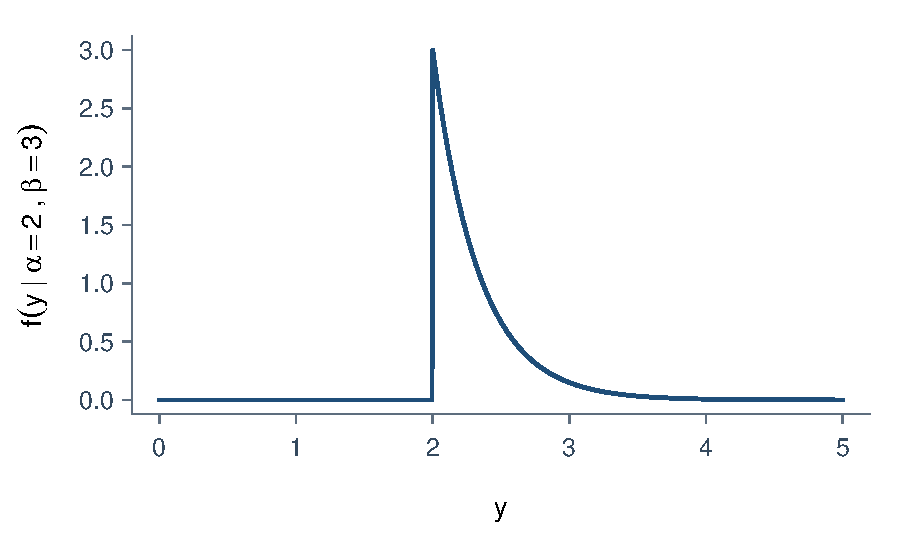
\includegraphics[width=0.62\linewidth]{ex16_density.pdf}\end{center}
$\alpha$ is a \textbf{minimum} (threshold, guarantee or lag time): no value can be smaller. $\beta$ is the \textbf{rate} of the exponential part: the time beyond $\alpha$ has mean $1/\beta$ (here $\frac13$). Example: the time until a customer's order is ready --- the kitchen needs at least $\alpha$ minutes, then random extra delay; or the lifetime of a component with a guaranteed minimum life.

\step{(b) Joint posterior.}
\[
p(\alpha,\beta\mid\mathbf Y)\propto\beta^n\exp\Big\{-\beta\sum_i(Y_i-\alpha)\Big\}\,\mathbb 1\big(\alpha\le Y_{(1)}\big)\cdot\mathbb 1(0<\alpha<c)\cdot\beta^{a-1}e^{-b\beta}.
\]
\step{(b) Full conditional of $\alpha$.}
Keep factors with $\alpha$: $\exp\{-\beta\sum(Y_i-\alpha)\}=\exp\{-\beta\sum Y_i\}\,e^{n\beta\alpha}$. So
\[
p(\alpha\mid\beta,\mathbf Y)\propto e^{n\beta\alpha}\quad\text{for }0<\alpha<u,\qquad u=\min(c,\,Y_{(1)}).
\]
This is a \emph{truncated exponential with a positive rate} (increasing density) --- not a common named family, but it is easy to sample by inverting its CDF:
\[
F(\alpha)=\frac{e^{n\beta\alpha}-1}{e^{n\beta u}-1}\ \Rightarrow\ \alpha=u+\frac{1}{n\beta}\log\big(U+(1-U)e^{-n\beta u}\big),\quad U\sim\dist{Uniform}(0,1).
\]
\why{Setting $F(\alpha)=U$ and solving gives $\alpha=\frac{1}{n\beta}\log\{1+U(e^{n\beta u}-1)\}$; we rewrite it in the form above (factoring out $e^{n\beta u}$) so that the computer never has to evaluate the enormous number $e^{n\beta u}$.}
\step{(b) Full conditional of $\beta$.}
\[
p(\beta\mid\alpha,\mathbf Y)\propto\beta^{n+a-1}\exp\Big\{-\beta\Big(b+\sum_i(Y_i-\alpha)\Big)\Big\}
\ \Rightarrow\ \beta\mid\alpha,\mathbf Y\sim\dist{Gamma}\Big(a+n,\ b+\sum_i(Y_i-\alpha)\Big)
\]
--- a common family.

\step{(c) Pseudocode.}
\begin{enumerate}[1.]
\item \textbf{Initial values}: $\alpha^{(0)}=\frac12\min(c,Y_{(1)})$ (safely inside the allowed range), $\beta^{(0)}=1/(\bar Y-\alpha^{(0)})$.
\item \textbf{For} $s=1,\dots,S$:
\begin{enumerate}[(i)]
\item $U\sim\dist{Uniform}(0,1)$, set $\alpha^{(s)}=u+\frac{1}{n\beta^{(s-1)}}\log\{U+(1-U)e^{-n\beta^{(s-1)}u}\}$;
\item $\beta^{(s)}\sim\dist{Gamma}\big(a+n,\ b+\sum_i(Y_i-\alpha^{(s)})\big)$.
\end{enumerate}
\item \textbf{Convergence}: run 3 chains from dispersed starting values (e.g.\ $\alpha^{(0)}$ near 0, middle and near $u$), discard the first 1{,}000 draws, check trace plots, $\hat R<1.01$ and ESS $>1{,}000$ for both parameters.
\end{enumerate}

\begin{sanity}
We tested the sampler on 40 simulated values with $\alpha=2$, $\beta=3$ (priors $\dist{Uniform}(0,5)$, $\dist{Gamma}(1,1)$): posterior means $\alpha=1.999$ (95\% CI 1.978--2.007) and $\beta=3.25$ (2.32--4.35). Both truths are recovered; $\alpha$ sits just below the smallest observation (2.007), exactly as the theory says.
\end{sanity}

\begin{answer}
(a) $\alpha$ = minimum value, $\beta$ = decay rate (mean excess $1/\beta$). (b) $\alpha\mid\cdot\propto e^{n\beta\alpha}$ on $(0,\min(c,Y_{(1)}))$ (truncated exponential, not a standard family but invertible); $\beta\mid\cdot\sim\dist{Gamma}(a+n,\ b+\sum(Y_i-\alpha))$. (c) Gibbs sampler above.
\end{answer}

\begin{takeaway}
The posterior of a threshold parameter is very concentrated (its uncertainty shrinks like $1/n$, not $1/\sqrt n$) and piles up against the smallest observation.
\end{takeaway}

% ================================================================= Exercise 17
\exercise{3.17 --- A nonlinear growth curve for \emph{T.\ rex}}

\begin{problem}{17}
Using the data (mass and age) provided in Listing 3.9, fit the following non-linear regression model:
\[
\texttt{mass}_i\sim\dist{Normal}(\mu_i,\sigma^2)\ \text{where}\ \mu_i=\theta_1+\theta_2\texttt{age}_i^{\theta_3},
\]
with priors $\theta_1\sim\dist{Normal}(0,100^2)$, $\theta_2\sim\dist{Uniform}(0,20000)$, $\theta_3\sim\dist{Normal}(0,1)$, and $\sigma^2\sim\dist{InvGamma}(0.01,0.01)$.
\begin{enumerate}[(a)]
\item Fit the model in JAGS and plot the data (age versus mass) along with the posterior mean of $\mu_i$ to verify the model fits reasonably well.
\item Conduct a thorough investigation of convergence.
\item Give three steps you might take to improve convergence.
\end{enumerate}
\end{problem}

\begin{restate}
Fit a power-law growth curve to 7 dinosaur fossils and investigate how well the MCMC sampler behaves.
\end{restate}

\begin{recall}
Data (Listing 3.9): mass $=(29.9,\ 1761,\ 1807,\ 2984,\ 3230,\ 5040,\ 5654)$ kg at ages $(2,\ 15,\ 14,\ 16,\ 18,\ 22,\ 28)$ years.
\end{recall}

\begin{keyidea}
For a \emph{fixed} $\theta_3$, the model is linear in $\theta_1,\theta_2$, so they (and $\sigma^2$) can be Gibbs-sampled; only $\theta_3$ needs Metropolis. But $\theta_2$ and $\theta_3$ trade off against each other (a larger exponent needs a smaller multiplier), which slows mixing.
\end{keyidea}

\solution
\step{(a) Model and fit.} JAGS code:
\begin{lstlisting}
model{
  for(i in 1:n){
    mass[i] ~ dnorm(mu[i], tau)
    mu[i] <- theta1 + theta2 * pow(age[i], theta3)
  }
  theta1 ~ dnorm(0, 1/100^2);   theta2 ~ dunif(0, 20000)
  theta3 ~ dnorm(0, 1);         tau ~ dgamma(0.01, 0.01)
}
\end{lstlisting}
Our sampler: Gibbs for $\theta_1$ (normal), $\theta_2$ (normal truncated to $(0,20000)$), $\sigma^2$ (inverse-gamma), random-walk Metropolis for $\theta_3$ (step 0.08, acceptance 40\%). Four chains $\times$ 40{,}000 iterations, 5{,}000 burn-in.
\begin{center}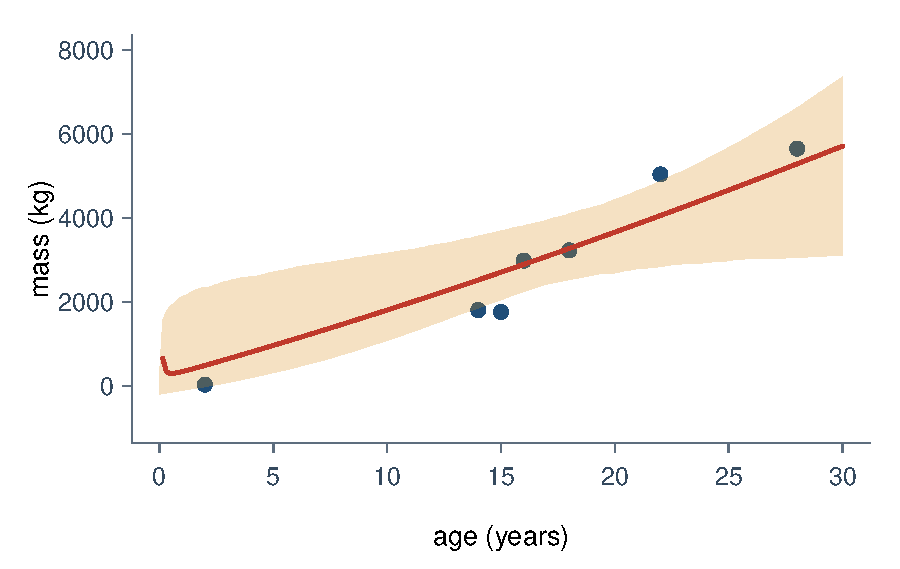
\includegraphics[width=0.66\linewidth]{ex17_fit.pdf}\end{center}
The posterior mean curve (red, with 95\% band) passes through the data: the fit is reasonable.
\begin{center}
\begin{tabular}{lcccc}\toprule
 & Mean & SD & 95\% interval\\\midrule
$\theta_1$ & $-16$ & 99 & $(-210,\ 179)$\\
$\theta_2$ & 354 & 825 & $(24,\ 2{,}139)$\\
$\theta_3$ & 1.06 & 0.41 & $(0.12,\ 1.67)$\\
$\sigma$ & 857 & 544 & $(360,\ 2{,}298)$\\\bottomrule
\end{tabular}
\end{center}
JAGS:
\JAGSexseventeen

\step{(b) Convergence investigation.}
\begin{center}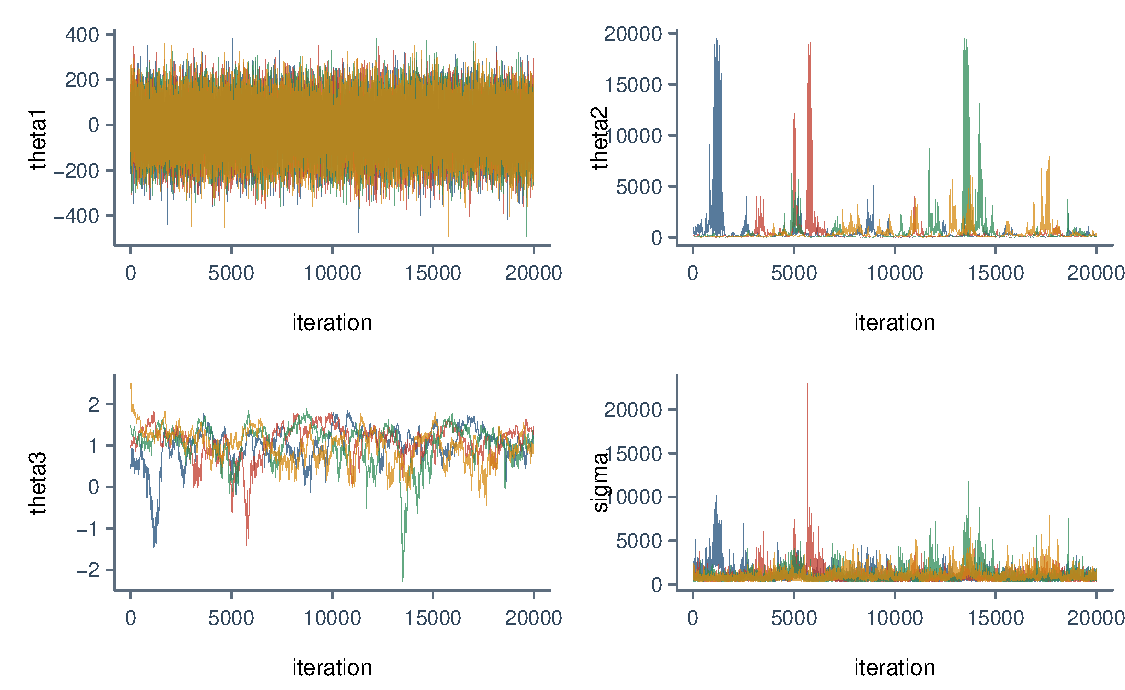
\includegraphics[width=0.98\linewidth]{ex17_traces.pdf}\end{center}
\begin{center}
\begin{tabular}{lccc}\toprule
 & $\hat R$ & ESS (of 140{,}000) & lag-1 autocorrelation\\\midrule
$\theta_1$ & 1.000 & 75{,}603 & 0.13\\
$\theta_2$ & 1.006 & 370 & 0.88\\
$\theta_3$ & 1.009 & 167 & 0.997\\
$\sigma$ & 1.005 & 410 & 0.56\\\bottomrule
\end{tabular}
\end{center}
$\theta_1$ mixes well; $\theta_2$ and $\theta_3$ mix very slowly (lag-1 autocorrelation 0.997 means each draw is almost a copy of the previous one), and the trace plots of $\theta_2$ show long excursions to large values. The chains agree ($\hat R<1.01$), but the ESS of 167 for $\theta_3$ from 140{,}000 draws is low: means are OK, tail quantiles are only roughly estimated. The cause is the strong dependence between $\theta_2$ and $\theta_3$ (correlation $-0.72$, and strongly nonlinear: the posterior is a curved ``banana'').

\step{(c) Three ways to improve convergence.}
\begin{enumerate}[1.]
\item \textbf{Reparameterise / centre}: write $\mu_i=\theta_1+\theta_2^*(\texttt{age}_i/20)^{\theta_3}$. Then $\theta_2^*$ is the mass at age 20, which is well determined whatever $\theta_3$ is, so $\theta_2^*$ and $\theta_3$ become nearly independent.
\item \textbf{Block updates}: propose $(\theta_2,\theta_3)$ jointly, e.g.\ a bivariate normal random walk with the posterior covariance estimated from a pilot run (adaptive Metropolis).
\item \textbf{Run longer and/or thin}, and use several chains with good starting values (e.g.\ from a nonlinear least-squares fit) to reach the bulk of the posterior quickly.
\end{enumerate}

\begin{answer}
(a) The posterior mean curve fits the 7 points well ($\theta_3\approx1.06$: roughly linear growth over this age range). (b) $\hat R<1.01$ but $\theta_2$, $\theta_3$ mix very slowly (ESS 370 and 167, lag-1 autocorrelation 0.88 and 0.997) because they are strongly dependent. (c) Reparameterise (centre age), block-update $(\theta_2,\theta_3)$, run longer chains with good inits.
\end{answer}

\begin{takeaway}
$\hat R\approx1$ is necessary but not sufficient: always look at ESS and autocorrelation too. Seven data points cannot pin down three curve parameters plus a variance --- slow mixing is often a symptom of weak identification.
\end{takeaway}

% ================================================================= Exercise 18
\exercise{3.18 --- A binomial with unknown number of trials}

\begin{problem}{18}
Assume the (overly complicated) model $Y|n,p\sim\dist{Binomial}(n,p)$ with prior distributions $n\sim\dist{Poisson}(\lambda)$ and $p\sim\dist{Beta}(a,b)$. The observed data is $Y=10$.
\begin{enumerate}[(a)]
\item Describe why convergence may be slow for this model.
\item Fit the model in JAGS with $\lambda=10$ and $a=b=1$. Check convergence and summarize the posterior of $n$, $p$ and $\theta=np$.
\item Repeat the analysis in (b) except with $a=b=10$. Comment on the effect of the prior distribution of $p$ on convergence for all the three parameters.
\end{enumerate}
\end{problem}

\begin{restate}
We see 10 successes but know neither the number of trials $n$ nor the success probability $p$. Only their product is really learned from the data. Show what that does to MCMC.
\end{restate}

\begin{recall}
From Chapter 1, Exercise 19: if $n\sim\dist{Poisson}(\lambda)$ and $Y\mid n\sim\dist{Binomial}(n,p)$, then $n-Y\mid Y,p\sim\dist{Poisson}(\lambda(1-p))$. And $p\mid n,Y\sim\dist{Beta}(a+Y,\ b+n-Y)$.
\end{recall}

\begin{keyidea}
The data identify $\theta=np$ (the expected count), not $n$ and $p$ separately. The posterior is a ridge along $np\approx10$: large $n$ with small $p$, or small $n$ with large $p$. A Gibbs sampler that moves one coordinate at a time zig-zags slowly along such a ridge.
\end{keyidea}

\solution
\step{(a) Why convergence may be slow.}
$n$ and $p$ are strongly negatively correlated in the posterior. Updating $n$ given $p$ (and then $p$ given $n$) only allows small moves along the ridge, so successive draws are highly autocorrelated. Also $n$ is discrete, so the sampler cannot make small adjustments.

\step{(b), (c) Gibbs sampler and results.}
Updates: $n=Y+M$ with $M\sim\dist{Poisson}(\lambda(1-p))$, then $p\sim\dist{Beta}(a+Y,\ b+n-Y)$. Three chains (starts $p=0.05,\ 0.5,\ 0.95$), 20{,}000 iterations, 1{,}000 burn-in.
\begin{center}
\small
\begin{tabular}{llcccccc}\toprule
Prior & & Mean & SD & 95\% interval & $\hat R$ & ESS (of 57{,}000) & lag-1 acf\\\midrule
\multirow{3}{*}{$a=b=1$} & $n$ & 11.99 & 1.99 & (10, 17) & 1.000 & 18{,}360 & 0.48\\
 & $p$ & 0.801 & 0.141 & (0.48, 0.99) & 1.000 & 18{,}135 & 0.50\\
 & $\theta$ & 9.40 & 1.25 & (6.6, 11.8) & 1.000 & 57{,}000 & $-0.07$\\\midrule
\multirow{3}{*}{$a=b=10$} & $n$ & 14.13 & 2.22 & (11, 19) & 1.000 & 39{,}512 & 0.17\\
 & $p$ & 0.589 & 0.091 & (0.41, 0.76) & 1.000 & 39{,}508 & 0.16\\
 & $\theta$ & 8.23 & 1.39 & (5.7, 11.1) & 1.000 & 57{,}000 & $-0.11$\\\bottomrule
\end{tabular}
\end{center}
\begin{center}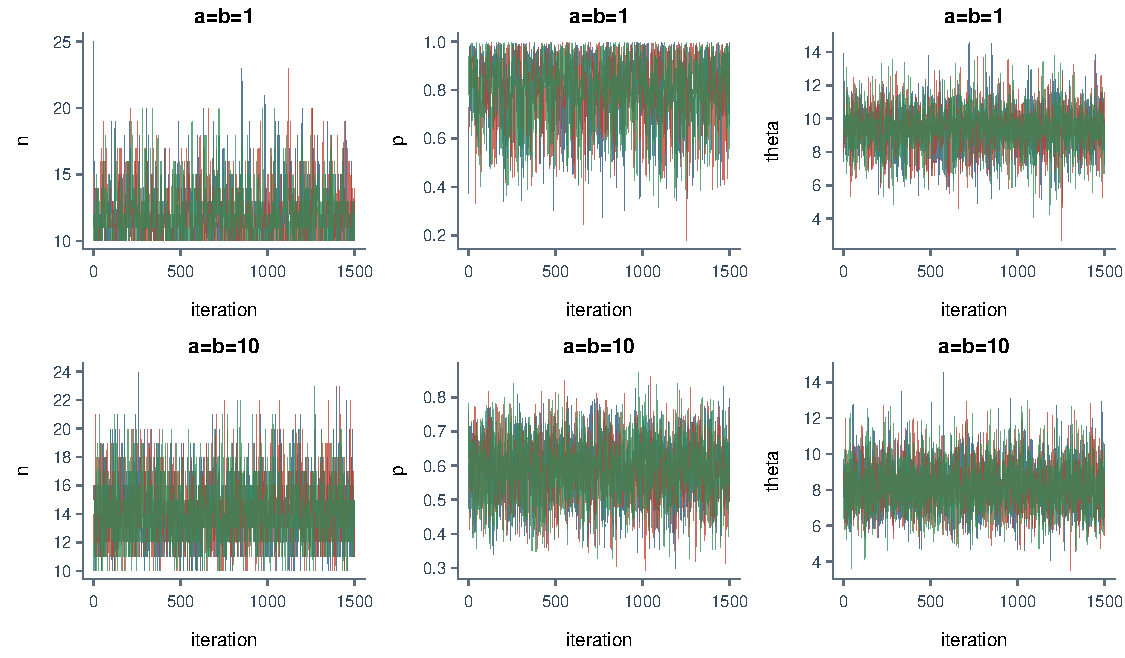
\includegraphics[width=0.98\linewidth]{ex18_traces.pdf}\end{center}
JAGS:
\JAGSexeighteen

\step{Comments.}
\begin{itemize}
\item With the flat prior ($a=b=1$), $n$ and $p$ have lag-1 autocorrelation $\approx0.5$ and only about a third of the draws are ``effective''. With $\lambda=10$ the prior already keeps $n$ near 10--17, so the problem is moderate here; with a vaguer prior on $n$ it would be much worse.
\item With $a=b=10$ the prior pins $p$ near 0.5, which cuts the ridge: the autocorrelation drops to 0.17 and the ESS doubles for both $n$ and $p$.
\item $\theta=np$ mixes perfectly in both cases (ESS = number of draws): the identified combination is always easy; only the unidentified directions are slow.
\end{itemize}

\begin{answer}
(a) Only $np$ is identified; the posterior ridge makes $n$ and $p$ highly correlated, so one-at-a-time updates move slowly. (b) $a=b=1$: $n\approx12$, $p\approx0.80$, $\theta\approx9.4$; converged but autocorrelated. (c) $a=b=10$: $n\approx14$, $p\approx0.59$, $\theta\approx8.2$; the informative prior on $p$ roughly halves the autocorrelation of $n$ and $p$, while $\theta$ mixes well in both cases.
\end{answer}

\begin{takeaway}
When parameters are weakly identified, an informative prior is not only a statement of knowledge --- it also makes computation easier. Report the identified quantity ($\theta$) with confidence; be cautious about $n$ and $p$ separately.
\end{takeaway}

% ================================================================= Exercise 19
\exercise{3.19 --- An over-parameterised hierarchical model}

\begin{problem}{19}
Consider the (overly complicated) model
\[
Y_i|\mu_i,\sigma_i^2\sim\dist{Normal}(\mu_i,\sigma_i^2)
\]
where $\mu_i\iid\dist{Normal}(0,\theta_1^{-1})$, $\sigma_i^2\sim\dist{InvGamma}(\theta_2,\theta_3)$ and $\theta_j\sim\dist{Gamma}(\epsilon,\epsilon)$ for $j=1,2,3$. Assume the data are $Y_i=i$ for $i=1,\dots,n$.
\begin{enumerate}[(a)]
\item Describe why convergence may be slow for this model.
\item Fit the model in JAGS with all four combinations of $n\in\{5,25\}$ and $\epsilon\in\{0.1,10\}$, and report the effective sample size for $\theta_1$, $\theta_2$ and $\theta_3$ for all four fits.
\item Comment on the effect of $n$ and $\epsilon$ on convergence.
\end{enumerate}
\end{problem}

\begin{restate}
Every observation gets its own mean \emph{and} its own variance. With one data point per pair, the model has far more parameters than information. See how this affects MCMC efficiency.
\end{restate}

\begin{keyidea}
Each $Y_i$ is a single number explained by two unknowns, $\mu_i$ and $\sigma_i^2$: a big $Y_i$ can be ``a big mean'' or ``a big variance''. The hyperparameters $\theta_2,\theta_3$ are learned only indirectly through the barely-identified $\sigma_i^2$ --- a recipe for slow mixing, especially with vague hyperpriors.
\end{keyidea}

\solution
\step{(a) Why convergence may be slow.}
\begin{itemize}
\item \textbf{Weak identification}: $\mu_i$ and $\sigma_i^2$ are confounded (one observation each).
\item $\theta_2$ (shape) and $\theta_3$ (scale) of the inverse-gamma are strongly correlated --- many (shape, scale) pairs give similar distributions for the $\sigma_i^2$.
\item With $\epsilon=0.1$ the hyperpriors are vague and heavy-tailed, allowing the sampler to wander into regions such as $\theta_3\to0$ where it gets stuck.
\end{itemize}

\step{Our sampler.} Gibbs for $\mu_i$ (normal), $\sigma_i^2$ (inverse-gamma), $\theta_1$ ($\dist{Gamma}(\epsilon+\frac n2,\ \epsilon+\frac12\sum\mu_i^2)$), $\theta_3$ ($\dist{Gamma}(\epsilon+n\theta_2,\ \epsilon+\sum\sigma_i^{-2})$), and Metropolis on $\log\theta_2$ (no conjugate form). 20{,}000 iterations, 2{,}000 burn-in, so the maximum ESS is 18{,}000.

\step{(b) Effective sample sizes.}
\begin{center}
\begin{tabular}{cc|ccc|ccc}\toprule
 & & \multicolumn{3}{c|}{ESS (of 18{,}000)} & \multicolumn{3}{c}{posterior median}\\
$n$ & $\epsilon$ & $\theta_1$ & $\theta_2$ & $\theta_3$ & $\theta_1$ & $\theta_2$ & $\theta_3$\\\midrule
5 & 0.1 & 1{,}054 & 168 & 146 & 0.089 & 1.57 & 0.001\\
5 & 10 & 7{,}532 & 2{,}550 & 11{,}641 & 0.874 & 0.81 & 1.10\\
25 & 0.1 & 12{,}513 & \textbf{7} & \textbf{55} & 0.004 & 1.83 & 0.049\\
25 & 10 & 4{,}164 & 3{,}206 & 10{,}558 & 0.915 & 0.29 & 1.49\\\bottomrule
\end{tabular}
\end{center}
JAGS:
\JAGSexnineteen

\step{(c) Effect of $n$ and $\epsilon$.}
\begin{itemize}
\item \textbf{$\epsilon$ matters most.} With $\epsilon=10$ the hyperpriors are informative ($\dist{Gamma}(10,10)$: mean 1, SD 0.32), which keeps $\theta_2,\theta_3$ in a sensible region; every ESS is in the thousands.
\item With vague hyperpriors ($\epsilon=0.1$) the variance hyperparameters mix terribly: ESS of 7 for $\theta_2$ when $n=25$ --- 20{,}000 iterations are worth about 7 independent draws. The posterior median of $\theta_3$ near 0 shows the chain drifting toward a degenerate region.
\item \textbf{More data does not automatically help.} Going from $n=5$ to $n=25$ improves $\theta_1$ (the $\mu_i$ are informative about their common spread), but not $\theta_2,\theta_3$, because each new observation also brings two new unknowns.
\end{itemize}

\begin{answer}
(a) Each observation has its own mean and variance (confounded), and the inverse-gamma shape/scale hyperparameters are strongly dependent. (b) See the ESS table. (c) Informative hyperpriors ($\epsilon=10$) give good mixing for all $\theta_j$; vague ones ($\epsilon=0.1$) give extremely poor mixing for $\theta_2,\theta_3$, and increasing $n$ does not cure it.
\end{answer}

\begin{takeaway}
If a model has (nearly) as many parameters as data points, expect MCMC trouble. Fixes: simplify the model (e.g.\ a common $\sigma^2$), use informative priors, or reparameterise.
\end{takeaway}

\end{document}
